% !TeX root = ./tesi.tex
% !TeX encoding = UTF-8 Unicode
% !TeX spellcheck = it_IT
% !TeX program = arara
% !TeX options = --log --verbose --language=it "%DOC%"

% arara: lualatex:      { interaction: batchmode }
% arara: frontespizio:  { interaction: batchmode, engine: lualatex }
% arara: biber
% arara: lualatex:      { interaction: batchmode }
% arara: lualatex:      { interaction: nonstopmode, synctex: yes }

\documentclass[%
  a4paper,                % formato di pagina A4
  12pt,                   % corpo del testo a 12pt
  % la dimensione 12pt automaticamente imposta \footnotesize a 10pt
  twoside,                % (oneside|twoside) documento a singola o doppia facciata,
  openright,              % (openany|openright) fa cominciare un capitolo nella successiva pagina a disposizione o sempre in una pagina destra
  % twocolumn,            % dà a LaTeX le istruzioni per comporre l'intero documento su due colonne
  titlepage,              % (titlepage|notitlepage) se dopo il titolo del documento debbaavere  inizio  una  nuova  pagina
  % fleqn,                % allinea le formule a sinistra rispetto a un margine rientrato
  % leqno,                % mette la numerazione delle formule a sinistra anziché a destra
  final                   % (draft|final) scelta tra bozza o finale, influenza il comportamento degli altri pacchetti
]{scrbook}

\usepackage{fancyvrb}       % fornisce l'ambiente VerbatimOut e modifica listati di codice
% \usepackage{minted}       % evidenzia la sintassi dei listati di codice; richiede pygments installato e shell-escape

\begin{VerbatimOut}{\jobname.xmpdata}
\Title{Titolo}
\Subject{Oggetto}
\Author{Niccolò Maltoni}
\Copyright{Questo documento è fornito sotto licenza Apache License, Version 2.0}
\CopyrightURL{https://opensource.org/licenses/Apache-2.0}
\end{VerbatimOut}

\usepackage[%
  english,italian             % definizione delle lingue da usare
]{varioref}                     % introduce il comando \vref da usarsi nello stesso modo del comune \ref per i riferimenti

\usepackage[a-1b]{pdfx}

%% Font
% non è necessario \usepackage[utf8]{inputenc} perché luaLaTeX accetta solo UTF-8
\usepackage{fontspec}
\setmainfont[%
  Ligatures=TeX               % abilita legature classiche di LaTeX
]{Latin Modern Roman}           % imposta il font con grazie per il testo principale
\setsansfont[%
  Ligatures=TeX               % abilita legature classiche di LaTeX
]{Latin Modern Sans}            % imposta il font senza grazie
\setmonofont[%
  Ligatures=TeX               % abilita legature classiche di LaTeX
]{Latin Modern Mono}            % imposta il font teletype monospaziato

%% Matematica
\usepackage{amsmath}
% non bisogna assolutamente invocare il pacchetto amssymb
\usepackage[%
  math-style=ISO              % per scrivere la matematica delle scienze sperimentali bisogna seguire le norme ISO
]{unicode-math}                 % implementazione di glifi Unicode per caratteri matematici
\setmathfont[%
  Ligatures=TeX               % abilita legature classiche di LaTeX
]{Latin Modern Math}
\usepackage[%
  output-decimal-marker={,},  % le convenzioni tipografiche italiane prevedono la virgola e non il punto
  binary-units                % abilita le espressioni per bit e byte
]{siunitx}                      % permette di definire numeri con unità di misura

%% Lingue
\usepackage[%
  strict=true,                % converte tutti i warning in errori
  autostyle=true,             % adatta continuamente lo stile delle virgolette alla lingua
  english=american,           % imposta lo stile per l'inglese
  italian=guillemets          % imposta lo stile per l'italiano
]{csquotes}                     % configura le virgolette secondo gli stnadard della lingua
\usepackage{polyglossia}
\setmainlanguage[%
  babelshorthands             % attiva il carattere " come switch per virgolettature etimologiche
]{italian}                      % imposta l'italiano come lingua principale
\setotherlanguage[%
  variant=american            % imposta la variante americana dell'inglese
]{english}                      % imposta l'inglese come lingua secondaria
% non è necessario \usepackage{indentfirst} perché con lualatex il rientro del primo capoverso è preimpostato

%% Altri pacchetti
\usepackage{graphicx}           % serve per includere immagini e grafici
\graphicspath{{res/fig}}      % importa la cartella res/fig/ come cartella da cui caricare le immagini
\usepackage{xcolor}             % permette di usare colori
% \usepackage{subcaption}       % serve per ottenere sottofigure
% \usepackage{caption}          % permette di controllare la formattazione delle didascalie
% \usepackage{adjustbox}        % permette di effettuare il crop delle immagini
% \usepackage{ctable}           % permette di migliorare la spaziatura dell'ambiente tabular standard
% \usepackage{flafter}          % impedisce alle figure di apparire prima della loro definizione nel testo
\usepackage{scrhack}            % risolve incompatibilità tra KOMA e pacchatti vari (float, listings, ...)
\usepackage{float}              % permette di forzare il posizionamento dell’oggetto nel punto in cui è situato con l’opzione H
\usepackage{afterpage}          % permette di eseguire qualcosa nella pagina successiva con \afterpage{...} (ad esempio, figure)
% \usepackage{placeins}         % permette di mettere delle barriere invalicabili per le figure con \FloatBarrier
\usepackage[%
  write,                      % (write|nowrite) genera o meno il file
  standard,                   % (standard|suftesi) specifica tipo di frontespizio
  normal,                     % (normal|sans) usa font con grazie anziché senza
  noinputenc,                 % non carica inputenc (poiché usa lualatex)
  % norules,                  % non vengono inseriti filetti nel frontespizio
  nouppercase,                % con questa opzione verrà rispettato il maiuscolo e il minuscolo
  driver=luatex               % imposta la chiamata di graphicx nel documento frn per l'uso di un driver diverso da dvips o pdftex
]{frontespizio}
\usepackage{geometry}           % permettte la modifica della gabbia del documento
\geometry{
  a4paper,                    % formato di pagina
  heightrounded,              % modifica di poco le dimensioni della gabbia per contenere un numero intero di righe
  hmargin=2.5cm,              % dimensioni margini destro-sinistro
  vmargin=2.5cm               % dimensioni margini superiore-inferiore
}
\usepackage{setspace}           % serve a fornire comandi di interlinea standard
\onehalfspacing{}             % imposta interlinea a 1,5 ed equivale a \linespread{1,5}

%% Definizioni di comandi e ambienti
%% Definisco un nuovo comando per enfatizzare il testo in inglese %%%%%%%%%%%
\newcommand{\engEmph}[1] {\emph{\foreignlanguage{english}#1}}

%% Aggiunge pagine bianche vuote %%%%%%%%%%%%%%%%%%%%%%%%%%%%%%%%%%%%%%%%%%%%
\newcommand{\clearemptydoublepage}{\newpage{\pagestyle{empty}%
%\cleardoublepage}}
\clearpage}}

%% Definisce l'environment abstract per la classe book %%%%%%%%%%%%%%%%%%%%%%
\newenvironment{abstract}%
  {\cleardoublepage%
    \thispagestyle{empty}%
    \null\vfill\begin{center}%
      \bfseries\abstractname\end{center}}%
  {\vfill\null}

\usepackage[%
  maxcitenames=2,             % massimo numero di nomi nelle citazioni
  mincitenames=2,             % minimo numero di nomi nelle citazioni
  maxbibnames=99,             % massimo numero di nomi nella blibliografia
  minbibnames=99,             % minimo numero di nomi nella blibliografia
  style=ieee,                 % imposta lo stile della blibliografia (numeric|alphabetic|authoryear|authortitle|verbose|...)
  giveninits=true,
  backend=biber               % specifica il backend per la bibliografia
]{biblatex}                     % si interfaccia con bibtex e biber per la bibliografia
\addbibresource{biblio.bib}
\usepackage[%
  % page,                     % Aggiunge una pagina con la scritta Appendices
  % toc,                      % Aggiunge un campo Appendices nell'indice
  titletoc,                   % Aggiunge la parola Appendice per ogni capitolo dell'appendice nell'indice
  title%                      % Aggiunge la parola Appendice per ogni capitolo dell'appendice
]{appendix}                     % modifica la gestione dell'appendice, e aggiunge l'ambiente appendices alternativo al comando \appendix
% \usepackage[htt]{hyphenat}    % permette la sillabazione dei blocchi di testo monospaziato
% \usepackage{enumerate}        % aggiunge un argomento opzionale che determina come comporre l’etichetta numerata delle liste

\usepackage{microtype}          % gestisce la microtipografia

% \usepackage{hyperref}         % gestisce tutte le cose ipertestuali del pdf; importato automaticamente
\hypersetup{%
  pdfpagemode={UseNone},
  hidelinks,                  % nasconde i collegamenti (non vengono quadrettati)
  hypertexnames=false,
  linktoc=all,                % inserisce i link nell'indice
  unicode=true,               % usa solo caratteri Latini nei segnalibri di Acrobat
  pdftoolbar=false,           % nasconde la toolbar di Acrobat
  pdfmenubar=false,           % nasconde il menu di Acrobat
  plainpages=false,
  breaklinks,
  pdfstartview={Fit},
  pdflang={it}
}

\usepackage[%
  english,italian,            % definizione delle lingue da usare
  nameinlink                  % inserisce i link nei riferimenti
]{cleveref}                     % permette di usare riferimenti migliori dei \ref e dei varioref

\usepackage{booktabs}         % permette di gestire le linee sulle tabelle in alternativa alle hbox

\begin{document}

  \frontmatter{}
  \pagenumbering{Roman}
  \pagestyle{empty}
  % !TeX root = ../../tesi.tex
% !TeX encoding = UTF-8 Unicode
% !TeX spellcheck = it_IT

\begin{Preambolo*}
  \usepackage{fontspec}
  \setmainfont[Ligatures=TeX]{Latin Modern Roman}
\end{Preambolo*}
\begin{frontespizio}
  \Universita{Bologna}        % aggiunge da sé “Università degli Studi di”.
  \Istituzione{%
    Alma Mater Studiorum --- Università di Bologna \\%
    Campus di Cesena%
  }
  \Divisione{Dipartimento di Informatica --- Scienza e Ingegneria}
  \Corso[Laurea magistrale]{Ingegneria e Scienze Informatiche}
  \Annoaccademico{2019--2020}
  \Titolo{Clustering di traiettorie in ambito Big Data}
  \Sottotitolo{Tesi in Data Mining}
  % \Preambolo{\renewcommand{\frontsmallfont}[1]{\small}}       % non viene stampata la matricola
  % \Preambolo{\renewcommand{\frontsmallfont}[1]{\small Matr.}} % abbrevia la matricola
  \Candidato[0000852918]{Federico~Naldini}
  \NCandidato{Presentata da}  % sostituisce la parola “Candidato”
  \Relatore{Prof.~Matteo~Golfarelli}
  \Correlatore{Dott.~Matteo~Francia}
  \Piede{%                    % sostituisce la scritta “Anno Accademico” nel piede
    III sessione di laurea \\%
    Anno Accademico 2019--2020%
  }
\end{frontespizio}

  % !TeX root = ../../tesi.tex
% !TeX encoding = UTF-8 Unicode
% !TeX spellcheck = it_IT

\clearemptydoublepage{}
\thispagestyle{empty}
\vspace*{20ex}
\begin{flushright}
    \begin{LARGE}
        \textbf{Parole chiave}\\
        \vspace{5ex}
    \end{LARGE}
    \begin{normalsize}
        \textbf{%
            Trajectory mining\\%
            \medskip
            Trajectory clustering\\%
            \medskip
            Big data%
        }
    \end{normalsize}
\end{flushright}
\vfill

  % !TeX root = ../../tesi.tex
% !TeX encoding = UTF-8 Unicode
% !TeX spellcheck = it_IT

\clearemptydoublepage{}
\null{}\vspace{\stretch{1}}
\begin{flushright}
    \textit{Dedica}
\end{flushright}
\vspace{\stretch{2}}\null{}

  % !TeX root = ../../tesi.tex
% !TeX encoding = UTF-8 Unicode
% !TeX spellcheck = it_IT

\begin{abstract}
  Abstract
\end{abstract}

  \tableofcontents

  \mainmatter{}
  \pagenumbering{arabic}
  \pagestyle{headings}

  \chapter{Clustering di traiettorie}\label{chapter:chapter1}
  
\section{Problematica}\label{sec:problem}
Uno degli obiettivi dell'analisi di dati di traiettoria è il \textit{clustering} (raggruppamento) di traiettorie simili.
Una traiettoria può essere considerata non solo come il tragitto percorso dall'oggetto che la genera,
ma anche come l'insieme delle attività, ciascuna corrispondente a una posizione, eseguite dal medesimo oggetto.
Lo scopo del clustering di traiettorie è quindi di scoprire quali condividono una certa similarità e quali invece no.
In tal modo è possibile identificare eventuali raggruppamenti di oggetti che hanno percorso assieme una certa frazione del loro percorso, oppure individuare eventuali
traiettorie differenti da tutte le altre.
Interpretando poi questi risultati partendo dalle traiettorie come insiemi di attività, è possibile ad esempio dedurre quali possano essere attività comuni e quali invece no.


\subsection{Clustering}\label{subsec:problem:clustering}
Il clustering, o analisi di raggruppamento, è una tecnica non supervisionata con lo scopo di aggregare i dati in \textit{cluster} o gruppi
tali che i dati all'interno di un gruppo siano più simili tra loro rispetto a quelli all'esterno\cite{liao2005clustering, zazzarro2009clustering}.

I metodi di clustering per elaborare dati statici di differenti tipologie sono cinque:

\begin{itemize}
  \item Metodi basati sul partizionamento:
  \item Metodi basati sulla gerarchia:
  \item Metodi basati sulla densità:
  \item Metdi basati su una griglia:
  \item metodi basati sul modello:
\end{itemize}




\subsection{Dati di traiettoria}\label{subsec:problem:trajectorydata}
Negli ultimi anni, la grande presenza di dipositivi in grado di catturare la posizione di un oggetto nel
tempo e le sue variazioni hanno prodotto enormi quantità di dati.
L'analisi di questi dati, resa possibile dalle moderne tecnologie Big Data, apre molteplici possibilità, come
ad esempio la ricerca dei flussi di traffico all'interno di un terriorio cittadino, oppure l'individuazione
dei luoghi più visitati da una certa categoria di utenti, o ancora il riconoscimento di gruppi di oggetti che si
muovono assieme all'interno di un certo spazio e tempo.
Dato il grande numero di potenziali fonti per i dati, è necessario ricondurre questi ultimi a una formulazione comune
così da poter sfruttare al meglio le loro potenzialità espressive.
La rappresentazione più basilare consiste nel considerare una traiettoria come l'insieme delle posizioni
spaziali dei punti che la compongono associando a ciascuno l'istante temporale in cui è stato registrato.
Questa formulazione prende il nome di traiettoria grezza (\textit{raw trajectory}), vedi~\cref{fig:chap-1:trajectory}
Andando a formalizzare quanto detto sopra:

\begin{figure}
  \centering
  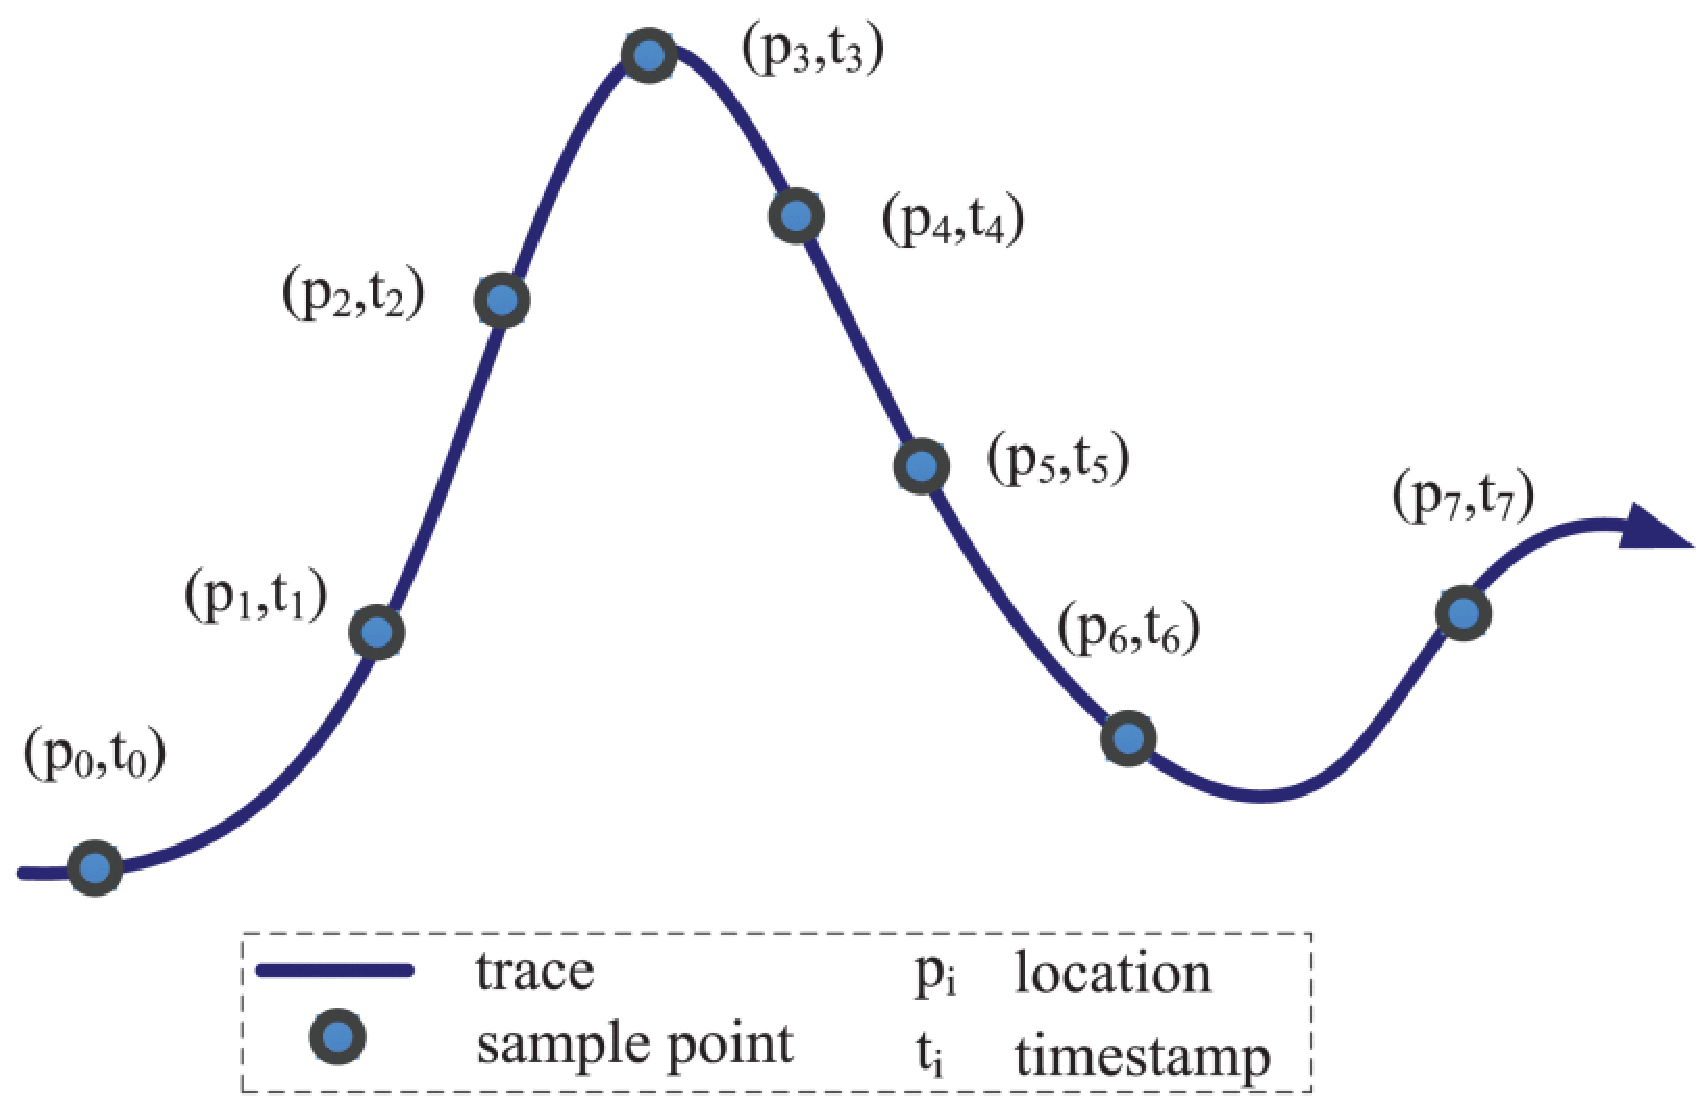
\includegraphics[scale=.5]{/sec-1/trajectory.pdf}
  \caption{Esempio di traiettoria,Fonte:\url{https://www.semanticscholar.org/paper/A-Survey-on-Trajectory-Data-Mining\%3A-Techniques-and-Feng-Zhu/a32f521442a540a6d1420526eaa68b3cab6b1d0d}}%
  \label{fig:chap-1:trajectory}
\end{figure}

\begin{definition}[Traiettoria]

  Si definisce una traiettoria grezza, o \textit{raw trajectory}, una sequenza temporale di punti \({p_{t}, p_{t'},\ldots, p_{t''}}\)
  tale che ogni punto \(p_{t}\) è composto da una coppia di coordinate spaziali \((latitude, longitude)\) e un tempo~\(t\).

\end{definition}

Questa basilare e semplice modalità di espressione può essere successivamente complicata, ad esempio adottando
una scala unica tra le diverse traiettorie per lo spazio e una per il tempo, oppure aggiungendo ulteriori informazioni, come ad esempio la direzione o attributi
dell'oggetto che la genera.

Per aumentare l'espressività della singola traiettoria, può essere utile definire il concetto di sotto-traiettoria, o \textit{subtrajectory}.
Intuitivamente una sotto-traiettoria non è altro che un segmento di una traiettoria relativo a un certo sottoinsieme dello spaziotempo coperto da quest'ultima.

\begin{definition}[Sottotraiettoria]

  Date due traiettorie \(TR\textsubscript{i}, TR\textsubscript{j}\) si definisce  \(TR\textsubscript{i}\) sottotraiettoria di \(TR\textsubscript{j}\) se \(\forall p_{t\textsubscript{i}} \in TR\textsubscript{i}, p_{t\textsubscript{i}} \in TR\textsubscript{j}\).

\end{definition}

Una volta definito che cos'è un dato di traiettoria, occorre mettere in chiaro che cosa distingue una traiettoria da un'altra.
Prendendo ad esempio il problema del clustering, sarebbe sbagliato tentare di applicare le stesse metriche di similarità anche ai dati di traiettoria
poiché gli oggetti in movimento producono spesso dati ad alta dimensionalità e con particolari correlazioni tra le dimensioni.
Il problema risulta quindi decisamente articolato: uno buona metrica di similarità deve tenere conto non solo dei singoli punti, ma anche della
traiettoria nella sua interezza, considerando anche la diversa lunghezza tra i due soggetti del confronto.
In letteratura sono presenti diversi metriche che possono essere impiegate nel confronto tra traiettorie:

\begin{itemize}

  \item \textbf{Distanza Euclidea.}
  La più semplice tra tutte le misure di stanza presentate, grazie alla sua complessità lineare permette di gestire dati ad alta dimensionalità.
  Date due traiettorie  \(T\textsubscript{i}\) e  \(T\textsubscript{j}\) di lunghezza \(n\) e dimensioni \(p\), la loro distanza euclidea si definisce come:

  \begin{equation}
    {D_E(T_{i}, T_{j}) = { {\frac{1}{n} } \sum_{k=1}^{n} {\sqrt{\sum_{m=1}^{p}{(a_{k}^{m} - b_{k}^{m})}^2}}}}
  \end{equation}

  La metrica tuttavia non è esente da difetti: è molto sensibile al rumore e richiede che le traiettorie siano uguali per numero di punti
  e dimensioni, inoltre anche l'intervallo di campionamento temporale deve coincidere. Questi limiti sono abbastanza difficili da
  aggirare quando si processa un dataset reale.

  Per superare questi problemi, sono disponibili diverse varianti della distanza euclidea: una su tutte è la \textit{Principal Component Analysis Plus Euclidean Distance} (PCA + distance)~\cite{zhang2006comparison}.
  Questa tecnica prima riduce le dimensioni spaziali ad una sola, successivamente esegue un'analisi PCA per convertire ogni traiettoria in
  \textit{k} coefficenti; a questo punto viene calcolata la distanza euclidea considerando i valori dei coefficenti individuati dall'analisi.
  Questa variazione mantiene gli stessi punti di forza della versione base della metrica, in più consente una maggior resistenza al rumore.



  \item \textbf{Distanza di Hausdorff.}
  La distanza di Hausdorff~\cite{chen2011clustering} misura quanto due traiettorie sono distanti l'una dall'altra.
  Date due traiettorie, per ogni punto di una viene calcolato il più vicino punto dell'altra e la distanza tra i due, il valore della distanza di Hausdorff
  corrisponde alla massima distanza calcolata nel passo precedente.~\cref{def:Hausdorff}
  \begin{equation} \label{def:Hausdorff}
    {D_{Hausdorff}(T_{i}, T_{j}) = \max{(h(T_{i}, T_{j}), h(T_{j}, T_{i}))}}~where~{h(T_{i}, T_{j}) = \max_{a \in T_{i}}{(\min_{b \in T_{j}}{(dist(a,b))})}}
  \end{equation}

  Nella formula \(h\) rappresenta la distanza di Hausdorff diretta, mentre \(d\) la distanza euclidea tra due punti.
  Il calcolo di entrambe le distanze dirette permette di gestire traiettorie con numero di punti differente tra loro.
  Questa metrica risulta robusta rispetto all'influenza causata da particolari distribuzioni di punti, ma allo stesso tempo è sensibile
  al rumore. Dalla formula~\cref{def:Hausdorff} è possibile definire la complessità computazionale della metrivca come \(O(m*n)\).


  \item \textbf{Distanza LCSS.}
  Longest Common Sub Sequence~\cite{rick2000efficient} affronta il problema con un approccio diverso: invece che calcolare la distanza fra i punti tra le due traiettorie, computa la
  più lunga sotto-sequenza.
  La lunghezza di quest'ultima determina la vicinanza,: più il valore è alto più le due traiettorie sono vicine.
  Essendo impossibile una coincidenza assoluta dei punti tra due traiettorie sono definite due soglie, \(\epsilon \) e \( \sigma \) che rispettivamente
  modellano la tolleranza rispetton all'asse x e y.
  LCSS può essere calcolata in modo ricorsivo, il suo tempo di computazione coincide con la diatnza di Hausdorff, inoltre consente una certa tolleranza rispetto
  alle deviazioni nei dati, ciò consente una buona efficenza nei dataset reali. Il maggior limite della metrica sta nella definizione dei parametri
  \(\epsilon \) e \( \sigma \) in problemi complessi.

  \item \textbf{Distnza DTW.}
  Dynamic time warping (DWT)~\cite{chen2005robust} pone il focus sulla dimensione temporale rispetto a quelle spaziali, come accadeva nelle metriche precedenti.
  Lo scopo è trovare l'allineamento ottimo tra due traiettorie dati certi vincoli.
  DWT resiste bene alle differenti lunghezze tra traiettorie: obbiettivo della misura è infatti ricercare il percorso a cui assimilare le traiettorie che abbia il minor coeficcente di distorsione,
  calcolato sulle trasformazioni subite dalle traiettorie.
  DWT assicura il rispetto dell'ordine tra i punti delle traiettorie, inoltre introducendo un principio di scaling locale della dimensione temporale,
  riesce a gestire scale temporali differenti tra le traiettorie.
  Tuttavia richiede continuità all'interno dei punti, è sensibile al rumore e a sottotraiettorie molto distanti tra loro.
  La complessità di questa misura è \(O(m*n)\).


  \item \textbf{Distanza di Fréchet.}
  La metrica di Fréchet~\cite{khoshaein2013trajectory} considera in contemporanea sia la dimensione temporale
  che quella spaziale durante il calcolo della distanza.
  Date due traiettorie di uguale lunghezza \(n\), si calcola la distanza euclidea tra i punti aventi stessa posizione all'interno delle due traiettorie:
  il valore più alto corrisponde alla distanza di Fréchet.
  Qualora le due traiettorie divergano come dimensioni, si eseguirà questo calcolo su tutte le possibili sotto-traiettorie di lunghezza \(n\) generabili
  dalla traiettoria più lunga.
  La complessità della misura nel caso peggiore è \(O(m*n)\).
  La distanza di Fréchet considera la traiettoria nella sua continuità, per questo motivo è molto sensibile agli outlier.


\end{itemize}





\section{Clustering di dati di traiettoria}\label{sec:problem:trajectoryclustering}

Come detto nella~\cref{sec:measure}, i dati di traiettoria sono molto più complessi
rispetto ai dati solitamente utilizzati con gli algoritmi di clustering tradizionali.
Occorre quindi definire modifiche di questi ultimi per riuscire a fare operazioni di clustering
efficienti, in quanto sarebbe impossibile catturare tutta la complessità dell'informazione con
tecniche pensate per dati a bassa dimensionalità.

Alla luce di quanto detto sopra, per il clustering di traiettorie sono individuabili i seguenti obbiettivi:

\begin{itemize}

  \item \textbf{Supporto alla dimensionalità dei dati}.
  Obbiettivo del clustering di traiettorie è la ricerca di cluster tenendo conto di tutte le informazioni presenti sui dati.
  Ognuno di questi attributi dovrà essere considerato nel momento in cui verranno portate avanti le operazioni di divisione e raggruppamento delle traiettorie.

  \item \textbf{Definizione di una metrica di similarità tra traiettorie}.
  Come presentato nella~\cref{sec:measure} il problema della similarità tra traiettorie è complesso e sono presenti diverse soluzioni.
  Scopo della ricerca è quello di individuare metriche che individuino le differenze tra le traiettorie in maniera affidabile e efficace.

  \item \textbf{Qualità dell'algoritmo}.
  L'algoritmo utilizzato nelle operazioni di clustering deve essere efficiente e scalabile, ad esempio impiegando apposite strutture dati per
  ridurre i tempi di accesso ai dati, oppure utilizzando le tecnologie di computazione Big Data per velocizzare l'esecuzione degli algoritmi.

\end{itemize}

Nonostante nessuno degli algoritmi di clustering tradizionali abbia tutte le caratteristiche espresse sopra, le idee alla loro base rimangono comunque
valide in buona parte dei casi.
Di conseguenza molti algoritmi pensati per i dati di traiettoria non sono che estensioni di quelli già noti in letteratura.

Gli algoritmi di clustering di traiettorie sono 
classificabili secondo la natura del dato in output
e sulla tipologia di clustering.
La natura del dato è direttamente collegata alle dimensioni considerate nelle operazioni di clustering:
la ricerca può essere condotta considerando solo la componente spaziale o includendo anche quella temporale.
La tipologia di clustering invece riguarda i cluster prodotti in output: algoritmi partizionanti 
produrranno cluster disgiunti, algoritmi di clustering sovrapposto cluster la cui intersezione non è vuota.

La \cref{tab:clus-alg} riassume i principali algoritmi che saranno trattati nelle sezioni successive alla luce della classificazione appena introdotta.
\begin{table}[H]
    \centering
   \begin{tabular}{||c c c||}
 \hline
 Algoritmo & Natura dei dati & Tipologia di clustering \\ [0.5ex] 
 \hline\hline
CB-SMoT & Spaziale & Sovrapposto \\ 
 \hline
CACT & Spaziale & Sovrapposto \\ 
 \hline
T-OPTICS & Spazio-temporale & Sovrapposto \\
 \hline
TraceMob & Spaziale & Partizionante \\
 \hline
 DSC & Spazio-temporale & Sovrapposto \\
 \hline

\end{tabular}
    \caption{Classificazione degli algoritmi di clustering di traiettorie trattati}
    \label{tab:clus-alg}
\end{table}

\begin{center}

\end{center}


\subsection{Algoritmi Spaziali}\label{subsec:problem:spatialalgorithms}
Le informazioni spaziali sono probabilmente la feature più importanti all'interno di un dato di traiettoria.
Analizzando come un oggetto si muove e i luoghi che visita possono essere ricavate una vasta serie di informazioni.
Negli anni vari algoritmi sono stati proposti per estrarre dai dati informazioni differenti tra loro.

Il primo ambito di ricerca sui dati spaziali riguarda i luoghi di maggior interesse, ovvero le posizioni
in cui sono passati un certo numero di oggetti all'interno del dataset.
A questa categoria appartiene il framework \textit{CB-SMoT} (Clustering Based Stop and Moves of Trajectories)~\cite{palma2008clustering}.
Questo algoritmo ricerca all'interno delle varie traiettorie considerando gli stop, ovvero segmenti in cui la velocità della traiettoria cala sotto una certa soglia o risulta uguale a zero.
Successivamente questi segmenti sono raggruppati in cluster usando una versione modificata di DBSCAN\@.
Tale versione dell'algoritmo si basa sulla velocità invece che sulla densità.
Infine ogni cluster viene confrontato con la mappa dell'area coperta dalle traiettorie e viene associato a uno specifico punto o area.
Questa associazione permette di interpretare meglio il risultato ottenuto dall'algoritmo.


Ancora è possibile estrarre da un insieme di dati di traiettorie, l'insieme delle strade più
frequentate; ciò diverge dal primo ambito presentato poiché la ricerca di un percorso risulta
più complessa rispetto a quella di un singolo punto: una strada infatti ha caratteristiche molto
più complesse di una singola località, come ad esempio una continuità nello spazio tra i vari punti che
la compongono.
\textit{CACT}~\cite{hung2015clustering} (Clustering and Aggregating Clues of Trajectories) è un possibile framework per
ricercare percorsi che rappresentino i comportamenti di una certa categoria di utenti.
L'idea dell'algoritmo è di definire una misura di similarità basata sugli indizi (\textit{clue}):
Un indizio è definibile come la vicinanza spazio-temporale di punti di traiettorie diverse che però condividono lo stesso comportamento.
Tale indizio costituisce una corrispondenza parziale di comportamento.
Sulla base della presenza di indizi simili, vengono costituiti cluster di traiettorie, che raggruppano queste ultime sulla base di un certo comportamento.
I cluster così ottenuti sono però ancora percorsi parziali, per determinare percorsi completi è necessario un ulteriore passo di ricerca di indizi e fusione dei cluster.

I due ambiti appena descritti partono dalla stessa interpretazione dei dati, cercando di eseguire una separazione tra le varie traiettorie sulla base delle proprietà dei singoli punti.
Un'alternativa a questa visione è presente nel clustering basato su forma (\textit{Shape Based Clustering}),
in cui i raggruppamenti sono basati sulla distribuzione dei punti piuttosto che sulle loro proprietà.
Questo approccio non si limita ad analizzare solo la dimensione spaziale, ma include nel determinare la forma di una traiettoria anche la sua dimensione temporale.


\subsection{Algoritmi Temporali}\label{subsec:problem:temporalalgorithms}

Come detto nella definizione di traiettoria (\cref{subsec:trajectory-definition})
le informazioni necessarie per definire un punto sono due: la componente spaziale e quella temporale.

Il tempo risulta più complesso da gestire rispetto allo spazio: è infatti praticamente impossibile
definire una scala temporale univoca all'interno di un dataset.
Essendo le traiettorie generate da diversi dispositivi GPS, è molto raro che questi condividano tra loro la frequenza
di campionamento, rendendo quindi difficile definire un ordine assoluto all'interno dell'area temporale
coperta dal dataset.
Oltre a ciò, la possibile adozione di scale cicliche per l'analisi del tempo rende necessario
introdurre ulteriore complessità negli algoritmi che supportano queste ricerche.

A differenza di quanto accade negli ambiti spaziali, la ricerca pone il suo accento
sull'interpretazione del tempo e la conseguente formazione dei cluster piuttosto che
solo su questo secondo ambito.

La maggior parte degli algoritmi riescono a gestire scale temporali assolute. Ad esempio
\textit{T-OPTICS}~\cite{nanni2006time} è una variante di OPTICS che impiega una metrica di similarità
adatta a individuare cluster considerando anche il tempo.
L'idea alla base dell'algoritmo è di ricercare il miglior intervallo temporale l'algoritmo OPTICS, appositamente modificato per la ricerca di traiettorie, individua i risultati migliori.
Sta all'utente specificare la lunghezza e il range dell'intervallo temporale: a seconda del periodo specificato i cluster individuati possono cambiare totalmente.
Come però affermato in un'indagine~\cite{mitsch2013survey} condotta nel 2013, esistono pochi framework in grado di gestire
scale temporali cicliche e la ricerca di pattern periodici.


\subsection{Altre categorie}\label{subsec:problem:othersalgorithms}
Nelle sezioni precedenti sono stati analizzati i dati di traiettoria sotto il profilo
spaziale e temporale, tuttavia sarebbe incompleto limitare la panoramica sul clustering di traiettorie
a queste due categorie.
Lo spazio-tempo sono indubbiamente le dimensioni più importanti all'interno di una traiettoria,
tuttavia, come affermato nella~\cref{subsec:problem:trajectorydata},
i dati che costituiscono quest'ultima hanno molte più dimensioni di quelle fin d'ora considerate.

Partendo da questo punto, sono state ideate altre categorie di clustering e raggruppamento dei dati
che sfruttano parte di queste informazioni in combinazione con gli attributi spazio-temporali,
i quali mantengono comunque un ruolo cruciale nella divisione delle traiettorie.

Una traiettoria è spesso composta da un grande numero di punti e processata nella sua completezza.
Questo però comporta che molti algoritmi tendano a ignorare caratteristiche locali
e di conseguenza mancare il riconoscimento di similarità tra diverse sotto-traiettorie.
Per risolvere questo problema, sono stati ideate tecniche per scomporre le traiettorie in segmenti più corti
e eseguire operazioni di clustering utilizzando le sotto-traiettorie così individuate.
Questa scomposizione non rende solo più agevoli le operazioni di clustering, ma cattura anche
quelle particolarità che sarebbero scartate processando le traiettorie nella loro interezza.
Gli algoritmi basati su questa idea sono definiti \textit{Partition and group based algorithm}.
Il focus principale di questa categoria è l'individuazione dei segmenti e
dei punti in cui ``spezzare'' la traiettoria originale.
Per risolvere questo problema sono state ipotizzate diverse soluzioni,
ad esempio il framework \textit{DST} (Distribuited Subtrajectory Clustering)~\cite{tampakis2019scalable} utilizza una metrica basata
sul cambio di densità nell'intorno dei punti della traiettoria per determinare le divisioni.
In generale questi framework hanno buoni risultati quando computano dataset di traiettorie
di lunghezze varie, inoltre resistono molto bene all'aumento del numero di punti da processare;
tuttavia non è banale individuare i segmenti ideali per catturare tutte le peculiarità
di una traiettoria.

Una traiettoria per definizione è composta da un insieme limitato di punti, tale numero
è direttamente collegato alla frequenza di campionamento del dispositivo GPS che registra
il moto in questione.
Nel caso in cui questa frequenza sia particolarmente alta, può succedere che si venga a creare
un certo grado di incertezza all'interno della traiettoria stessa: dati due punti consecutivi
\(p_{1}\) e \(p_{2}\) registrati agli istanti \(t_{1}\) e \(t_{2}\), non c'è modo di sapere con certezza quali
movimenti abbia eseguito l'oggetto tra  \(t_{1}\) e \(t_{2}\).
Questa mancanza di informazioni ha dato origine a una categoria di algoritmi,
chiamati \textit{Uncertain Trajectory Clustering algorithm}, con lo scopo direttamente
creare cluster tenendo conto di questa variabilità nel singolo dato.
L'introduzione dell'incertezza all'interno di questi framework consente loro di poter
processare anche dataset in cui sono presenti numerosi outlier e i dati in generale
hanno molto rumore.
Un' altra applicazione di questa categoria è nella deanonimizzazione dei dati: grazie
alla ricerca di cluster incerti è possibile invertire in parte il processo di anonimizzazione
dei dati all'interno di un dataset e dedurre così informazioni nascoste, come
ad esempio il gruppo di appartenenza di un certo oggetto sulla base dei suoi movimenti.

Nessuno degli approcci fino ad ora trattati ha posto la propria attenzione sulle informazioni non
strettamente spazio-temporali, come ad esempio la misura della velocità di un oggetto
o la direzione del suo movimento.
Gli algoritmi basati sulla semantica mettono in primo piano queste informazioni rispetto a quelle
spazio-temporali, ottenendo risultati altrimenti impossibili da raggiungere.
Ad esempio considerando velocità e accelerazione è possibile determinare quali possano
essere i punti in cui una certa categoria di utenti tende a fermarsi più spesso~\cite{zheng2008understanding},
oppure capire quale sarà il percorso di un utente assegnato a una certa categoria sulla base
di come si sono mossi gli altri appartenenti al medesimo gruppo~\cite{ying2011semantic}.
Questa categoria è in continua crescita, con algoritmi sempre più complessi e che sfruttano sempre di
più l'interezza dell'informazione offerta dal singolo dato.









\subsection{Applicazioni e limiti}\label{subsec:problem:applicationandlimits}

\section{Comovement patterns}\label{sec:problem:comovements-pattern}

\section{Frequent Itemset Mining}\label{sec:problem:frequent-itemset-mining}



  \chapter{L'algoritmo G.C.M.P}\label{chapter:chapter2}
  
\section{Definizione di pattern di co-movimento}\label{sec:comovement-definition}
Un'analisi cruciale che può essere eseguita su un dataset di traiettorie è sicuramente la ricerca di oggetti che si muovono assieme.
Come detto nella \cref{subsec:fim-trajectory}, il mining di traiettorie pone l'attenzione sulla sul percorso e non sugli oggetti che ne fanno parte.
L'analisi dei gruppi di oggetti è molto simile nelle modalità a quella dei percorsi/luoghi frequenti, tuttavia le potenzialità informative sono totalmente diverse.
Analizzando i gruppi di oggetti si può vedere come questi variano nello spazio e nel tempo, ad esempio vedendo in quali gruppi un oggetto viaggia e per quanto.
Questa analisi può portare a diversi risultati, ad esempio sulla base di regolarità di certi gruppi di viaggio è possibile dedurre informazioni sulle modalità di viaggio di un utente.
Ancora la ricerca di gruppi di oggetti in movimento può fornire informazioni sul comportamento comune e quindi la natura di un certo gruppo: ad esempio un gruppo di molti utenti che viaggia insieme per un lungo periodo di tempo nel perimetro di una città potrebbe essere collegato a un tour turistico, al contrario un gruppo numeroso che viaggia assieme per un breve periodo potrebbe indicare un insieme di persone che stanno viaggiando su un mezzo pubblico.

Un \textit{co-movement} pattern~\cite{zheng2015trajectory} individua un gruppo di oggetti che si sono mossi assieme
per un certo tempo.
L'appartenenza a tale gruppo è determinata solitamente dalla vicinanza nello spazio.
La ricerca di questi pattern di movimento include diversi parametri che definiscono le caratteristiche dei gruppi individuati.
Varie tipologie di cluster sono state definite in letteratura sulla base dell'adozione e configurazione di questi parametri.

Prima di scendere nel dettaglio sui singoli pattern, occorre definire gli elementi principali del problema.
Innanzitutto dato un dataset di traiettorie \(TR_{db} = \{tr_{1}, \ldots, tr_{n}\} \), da questo viene derivato il dataset
degli oggetti che hanno generato quelle traiettorie, \(O_{db} = \{ o_{1}, \ldots, o_{m} \}, m \leq n\)
e un dataset contenente tutti i possibili istanti temporali del primo dataset
\(T_{db} = \{t_{1}, \ldots, t_{k}\} \).
In generale, nella ricerca di co-movement pattern si ricerca un gruppo di oggetti \(O = \{ o_{1}, \ldots, o_{p} \}, O \subseteq O_{db} \)
tale che il corrispondente \(T = \{t_{1}, \ldots, t_{j}\} T \subseteq T_{sb}\), definito come l'insieme degli istanti in cui gli oggetti di \(O\) sono vicini, goda di certe proprietà, come
ad esempio una lunghezza minima, oppure una continuità all'interno del tempo.
Due parametri comuni a tutti i pattern di movimento sono \(m\), che individua una
soglia minima per la dimensione di \(O\) e \(k\), limite inferiore al numero
di istanti temporali in cui il gruppo in questione è considerato vicino.
La \cref{tab:co-movement-pattern} riassume i principali vincoli che saranno adoperati nella ricerca di pattern.

\begin{table}[H]
    \centering
   \begin{tabular}{||c c||}
 \hline
     Parametro & Vincolo espresso\\ [0.4ex] 
 \hline\hline
     \(m\) & dimensione minima del gruppo \\ 
 \hline
    \(k\) & minimo numero di istanti temporali in cui il gruppo è stato assieme \\ 
 \hline
     \(l\) & lunghezza minima di ogni sotto-sequenza continua di \(T\)\\ 
 \hline
\end{tabular}
    \caption{Parametri per la ricerca di pattern di co-movimento e il loro significato}
    \label{tab:co-movement-pattern}
\end{table}

I pattern di movimento possono essere suddivisi in due categorie a seconda dell'algoritmo di clustering utilizzato per riconoscere quali punti siano vicini e quali no.
Se viene impiegato un clustering basato sulla distanza, allora si parla di \textit{distance based pattern} (pattern basati sulla distanza), mentre se viene utilizzato un algoritmo basato sulla densità, allora si parla di \textit{density based pattern}.
Per semplicità nelle tipologie di pattern presentate d'ora in poi si fa riferimento a pattern basati sulla densità.

Il primo pattern di movimento individuabile alla luce dei vincoli è \textit{swarm}~\cite{li2010swarm}.
In maniera informale, swarm ricerca gruppi di \(m\) oggetti che hanno viaggiato assieme per almeno \(k\) istanti temporali senza porre alcun ulteriore vincolo.
Uno swarm può essere definito come segue:

\begin{definition}[Swarm]\label{definition:swarm}

  Una coppia \( \{ O, T \} \) si definisce swarm se:

  \begin{center}

    \(
      \begin{cases}
         \forall t \in T,\exists c \; t.c \; O \in c \\
         |O| \geq m \\
         |T| \geq k

      \end{cases}
      \)

  \end{center}
\end{definition}

La~\cref{definition:swarm} formalizza i seguenti vincoli:
ad ogni istante di \(T\) gli oggetti di \(O\) devono appartenere a uno stesso cluster,
il gruppo deve essere poi rilevante dal punto di vista degli elementi (\(m\)) e del tempo trascorso
(\(k\)).
Per quanto riguarda il primo vincolo, è possibile utilizzare varie metriche per fare clustering
sulla dimensione spaziale del dataset, tuttavia l'algoritmo più utilizzato per la ricerca di swarm
è DBSCAN (\cref{sec:clustering}).


Il concetto di swarm può essere ulteriormente raffinato in quello di \textit{closed swarm}:
un closed swarm intuitivamente si definisce allo stesso modo di uno swarm, ma con l'ulteriore
vincolo di considerare la massima sequenza di istanti in cui gli oggetti dentro \(O\) risultano vicini
tra di loro (chiusura rispetto al tempo) oppure il numero massimo di oggetti dato un certo \(T\) (chiusura rispetto agli oggetti).
Formalmente, ciò è espresso nella~\cref{definition:closed-swarm}

\begin{definition}[Closed Swarm]\label{definition:closed-swarm}

  Una coppia \( \{ O, T \} \) si definisce closed swarm se:

  \begin{center}

    \(
      \begin{cases}
         \{ O, T \} \; risulta \; swarm   \\
         \nexists O' \; t.c. \;  \{ O \cup O', T \} risulta \; swarm   \\
         \nexists T' \; t.c. \;  \{ O, T \cup T' \} risulta \; swarm
      \end{cases}
    \)

  \end{center}

\end{definition}

Com'è possibile vedere in~\cref{fig:chap-1:SwarmExample} (Fonte:~\cite{phan2016all}), la ricerca di swarm produce riconosce
il gruppo \( \{ o_{1}, o_{2}\} \) in quanto i due oggetti risultano avere viaggiato vicini per almeno
tre istanti temporali (\(t_{1}, t_{3}, t_{4}\)).

\begin{figure}
  \centering
  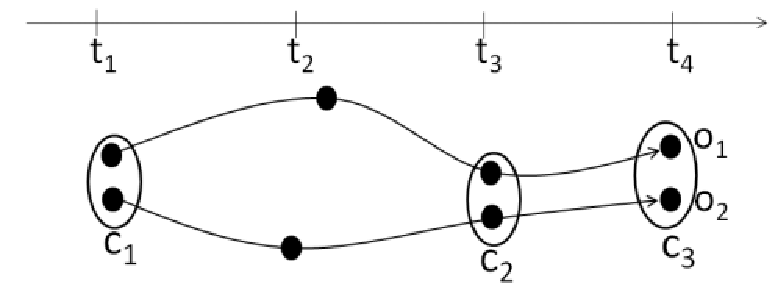
\includegraphics[width=\textwidth]{/sec-2/SwarmExample.pdf}
  \caption{Ricerca di swarm su un dataset fissati \(m=2\) e \(k=3\), Fonte:\cite{DBLP:journals/ijitdm/PhanPT16}}%
  \label{fig:chap-1:SwarmExample}
\end{figure}


Entrambi i pattern appena presentati rilassano al massimo i vincoli sul tempo,
accettando gruppi aventi istanti temporali parecchio distanti gli uni dagli altri.
Un tipo di analisi che aggiunge un rigido vincolo sulla continuità degli istanti temporali è
la ricerca di \textit{convoy}~\cite{jeung2008convoy}: un convoy per definizione è un raggruppamento di oggetti \(O\) in cui
tutti gli istanti in \(T\) sono consecutivi, mantenendo i precedenti vincoli sulle dimensioni del
gruppo e sul tempo trascorso assieme.

\begin{definition}[Convoy]\label{definition:convoy}
  Una coppia \( \{ O, T \} \) si definisce convoy se:
  \begin{center}
    \(
      \begin{cases}
         \{ O, T \} \; risulta \; swarm   \\
      \forall t_{i} \in T, t_{i+1} = t_{i} + 1
      \end{cases}
    \)

  \end{center}
\end{definition}

Convoy utilizza un algoritmo basato su densità, come ad esempio DBSCAN, per determinare
la vicinanza o meno di due oggetti in base all'appartenenza a un certo cluster ad ogni
\(t_{i}\).
Qualora si voglia adottare un algoritmo basato sulla distanza per determinare la vicinanza, allora i
pattern individuati sono chiamati \textit{flock}~\cite{benkert2008reporting} pattern.
La~\cref{fig:chap-1:ConvoyExample} (Fonte:~\cite{phan2016all}) mostra un esempio di ricerca di convoy: fissati \(m=2\)
e \(k=3\), risulta come pattern valido \( \{ o_{1}, o_{2}\} \),
\( \{ o_{1}, o_{2}, o_{3}\} \) viene scartato in quanto non soddisfa il vincolo di continuità
sugli istanti temporali.

\begin{figure}
  \centering
  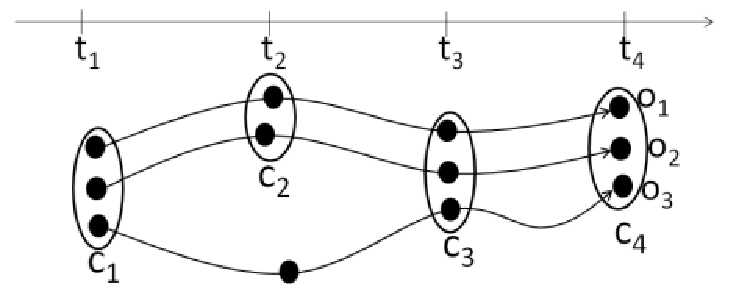
\includegraphics[width=\textwidth]{/sec-2/ConvoyExample.pdf}
  \caption{Ricerca di convoy su un dataset fissati \(m=2\) e \(k=3\), Fonte:\cite{DBLP:journals/ijitdm/PhanPT16}}%
  \label{fig:chap-1:ConvoyExample}
\end{figure}

Convoy e swarm rappresentano i due casi limite per quanto riguarda la rigidità dei vincoli temporali:
swarm rilassa totalmente la continuità mentre convoy esige una rigidità assoluta nella sequenza
degli istanti temporali.
Una via di mezzo tra i due estremi è individuata nel pattern \textit{group}~\cite{wang2006efficient}.
Un pattern group individua un insieme di convoy disgiunti nel tempo relativi allo stesso gruppo di oggetti \(O\);
interpretando ogni convoy come un singolo punto temporale \(t_{s}\), un pattern group può essere visto come uno swarm
di convoy.
Ognuno dei singoli punti così individuati dovrà risultare come valido convoy, si definisce
il parametro \textit{l} come la lunghezza di istanti condivisi in ognuno dei punti individuati.
Il valore di \(k\) per lo swarm così individuato indica il numero minimo di convoy necessari per il riconoscimento di group,
solitamente tale valore è fissato a \(1\).

\begin{definition}[Group]\label{definition:group}
  Definito \(T\) come l'insieme totale di istanti in cui gli oggetti di \(O\) sono vicini,
  \(T_s\) come l'insieme delle sotto-sequenze continue e disgiunte \(T' \subseteq T\)
  una coppia \( \{ O, T_{s} \} \) si definisce group se:
  \begin{center}
    \(
      \begin{cases}
         \{ O, T_{s} \} \; risulta \; swarm   \\
      \forall t_{s} \in T_{s}, \; |t_{s}| \geq l
      \end{cases}
    \)

  \end{center}
\end{definition}

\begin{figure}
  \centering
  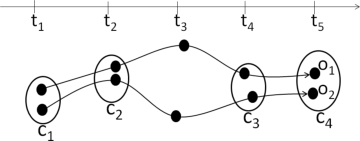
\includegraphics[width=\textwidth]{res/fig/sec-2/Group.pdf}
  \caption{Ricerca di group su un dataset fissati \(m=2\) e \(l=2\), Fonte:\cite{DBLP:journals/ijitdm/PhanPT16}}%
  \label{fig:chap-1:GroupExample}
\end{figure}

La \cref{fig:chap-1:GroupExample} contiene un esempio di ricerca di pattern group, com'è possibile vedere il parametro \(k\) non è considerato nella ricerca.

Group introduce la possibilità di ricercare gruppi con una continuità rilassata, tuttavia
non pone nessun vincolo sul numero complessivo di istanti necessari per considerare un pattern interessante.
Per integrare questo parametro, è stato definito il pattern \textit{platoon}~\cite{li2015efficient}.
Questo approccio interpreta diversamente il valore di \textit{k} rispetto a quanto fatto in
group: se in quest'ultimo approccio \(k\) indicava il numero di convoy necessari per individuare
un raggruppamento valido, ora \(k\) indica il numero di istanti assoluti necessari per
un gruppo valido.
In termini formali, il pattern platoon può essere definito come segue:

\begin{definition}[Platoon]\label{definition:platoon}
  Definito \(T\) come l'insieme totale di istanti in cui gli oggetti di \(O\) sono vicini,
  \(T_s\) come l'insieme delle sotto-sequenze continue e disgiunte \(T' \subseteq T\)
  una coppia \( \{ O, T \} \) si definisce platoon se:
  \begin{center}
    \(
      \begin{cases}
         \{ O, T \} \; risulta \; swarm   \\
      \forall T' \in T_{s}, \; |T'| \geq l
      \end{cases}
    \)
  \end{center}
\end{definition}

\begin{figure}
  \centering
  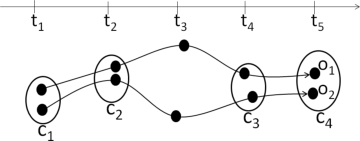
\includegraphics[width=\textwidth]{res/fig/sec-2/Group.pdf}
  \caption{Ricerca di Platoon con \(m = 2\), \(k = 3\), \(l=2\), Fonte:\cite{DBLP:journals/ijitdm/PhanPT16}}%
  \label{fig:chap-1:PlatoonExample}
\end{figure}

Com'è possibile vedere nella \cref{fig:chap-1:PlatoonExample}, in questo caso i risultati di platoon e group coincidono.
Tuttavia non è sempre così: confrontando l'applicazione dei pattern appena descritti a uno stesso dataset, la 
\cref{fig:chap-1:AllExample} mostra
quali sono le differenze, a parità di valori di \(m, k \) e \(l\), tra i diversi pattern di movimento.
Dalla figura in questione emergono chiaramente le differenze tra i gruppi individuati dai
vari pattern: ad esempio group riconosce \( \{ o_{3}, o_{4}, o_{5}\} \) negli istanti \( \{ 1, 2 \} \)
poiché la lunghezza di tale sotto-sequenza risulta uguale ad \(l\); platoon invece spezza
il raggruppamento in \( \{ o_{3}, o_{4} \}, \{ o_{4}, o_{5} \} \) poiché quest'ultimo non
avrebbe rispettato il vincolo sulla lunghezza minima degli istanti \(k\).
Convoy e Swarm invece riconoscono i pattern aventi una continuità assoluta in un caso,
totalmente assente nell'altro.
Entrambi ignorano il valore del parametro \(l\).

\begin{figure}
  \centering
  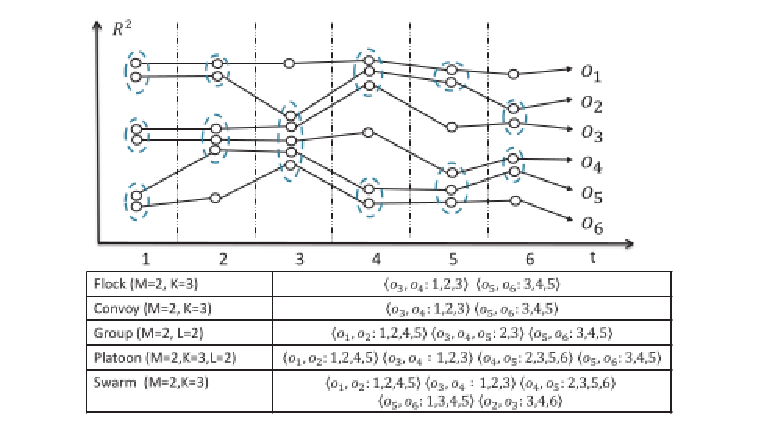
\includegraphics[width=\textwidth]{/sec-2/AllExamples.pdf}
  \caption{Ricerca dei principali pattern di movimento su un dataset fissati \(m=2\), \(k=3\) e \(l=2\), Fonte:~\cite{DBLP:journals/pvldb/FanZWT16}}%
  \label{fig:chap-1:AllExample}
\end{figure}

La \cref{tab:co-movement-pattern-list} riassume i pattern di co-movimento appena presentati in relazione ai vincoli espressi.

\begin{table}[H]
    \centering
   \begin{tabular}{||c c c c||}
 \hline
     Pattern & Dimensione del gruppo & Numero di istanti & Continuità \\ [0.4ex] 
 \hline\hline
     swarm & \(m\) & \(k\) & - \\ 
 \hline
    closed swarm & \(m\) & \(k\) & - \\ 
 \hline
     convoy & \(m\) & \(k\) & globale \\ 
  \hline
     group & \(m\) & - & locale \\
  \hline
    platoon & \(m\) & \(k\) & locale \\ 
 \hline
\end{tabular}
    \caption{Parametri per la ricerca di pattern di co-movimento e il loro significato}
    \label{tab:co-movement-pattern-list}
\end{table}


\section{L'algoritmo SPARE}\label{sec:gcmp}
Come può essere visto nella sezione precedente, sono presenti varie tipologie di pattern di co-movimento.
Platoon risulta il più generale tra tutti quelli appena esposti, essendo in grado di rappresentare gli altri con certe combinazioni specifiche di parametri.
I vari pattern quindi non sono totalmente separati tra di loro, ma possono essere ricondotti a una formulazione comune.

Un problema che affligge tutti i pattern di movimento in cui la continuità nel tempo è locale è l'anomalia \textit{loose-connection}, o della connessione interrotta.
Questa anomalia si presenta quando un gruppo di oggetti viaggia assieme per brevi periodi continui intervallati da lunghe distanze in cui il gruppo si rompe.
La \cref{fig:chap-2:loose-couple-anomaly} mostra un esempio di anomalia: gli oggetti \(o_1, o_2\) viaggiano assieme negli istanti \(1,2,3~\text{e}~102, 103, 104\).
Questo gruppo costituirebbe un platoon valido impostando \(m = 2, k = 4, l = 3\), tuttavia i quasi cento istanti temporali tra le due sotto-sequenze continue portano a pensare che
la relazione tra queste sia debole, essendo molto distanti nel tempo.

\begin{figure}
    \centering
    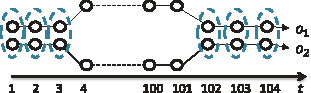
\includegraphics[width=\textwidth]{res/fig/sec-2/LooseCoupleAnomaly.pdf}
    \caption{Anomalia di connessione interrotta nel pattern \(o_1, o_2\): costituiscono un platoon valido ma le sotto-sequenze sono a 98 istanti l'una dall'altra, Fonte: \cite{DBLP:journals/pvldb/FanZWT16}}%
    \label{fig:chap-2:loose-couple-anomaly}
\end{figure}

GCMP, o General Co-Movement Pattern, è un astrazione per modellare varie tipologie di pattern di movimento.
Questa si occupa non solo di modellare i principali pattern di movimento con una tecnica univoca, ma anche di risolvere l'anomalia della connessione interrotta.

A questo proposito viene aggiunto il parametro \(g\), o gap temporale, agli altri parametri individuati nella \cref{sec:comovement-definition}.
Dati due istanti temporali \( t_1, t_2\), \(g\) rappresenta la massima distanza in termini di istanti tra questi.
Questo ulteriore vincolo permette di limitare l'anomalia della connessione interrotta: ad esempio nel caso descritto in \cref{fig:chap-2:loose-couple-anomaly} basta specificare \(g = 10\)
per scartare il pattern.

GCMP è quindi in grado di modellare pattern di movimento aventi le seguenti proprietà:

\begin{itemize}
    \item \textbf{Chiusura}.
    Dato un gruppo di oggetti \(O\) in una sequenza temporale \(T\), ogni oggetto \(o_i\) risulta vicino ad ogni altro oggetto di \(O\) ad ogni istante temporale \(t_i \in T\).
    
    \item \textbf{Importanza}.
    Definito un valore di \(m\), il numero di oggetti in \(O\) deve essere maggiore o uguale a \(m\).
    
    \item \textbf{Durata}.
    Definito un numero minimo di istanti temporali \(k\) per considerare un gruppo interessante, \(|T| \geq k \).
    
    \item \textbf{Consecutività}.
    Definito \(l\) come il valore minimo di consecutività locale, ogni sotto-sequenza continua di \(T\) deve risultare maggiore o uguale a \(l\).
    Una sequenza che rispetta questa proprietà viene detta \textit{L-consecutive}, o consecutiva rispetto a \(l\).
    
    \item \textbf{Connessione}.
    Definito \(g\) come il massimo gap tra due punti nel tempo, deve valere che \( \forall t_i \in T, d_t{(t_i, t_{i + 1}) \leq g}\).
    Una sequenza che rispetta questa proprietà viene detta \textit{G-connected}, o connessa rispetto a \(g\).
\end{itemize}

GCMP è quindi in grado di modellare tutti i pattern di co-movimento fin d'ora descritti variando i parametri come descritto nella \cref{tab:co-movement-pattern-gcmp}:

\begin{table}[H]
    \centering
   \begin{tabular}{||c c c c c||}
 \hline
     Pattern & M & K & L & G \\ [0.4ex] 
 \hline\hline
     swarm & \(m\) & \(k\) & 1 & \(\infty\) \\ 
 \hline
    closed swarm & \(m\) & \(k\) & 1 & \(\infty\) \\ 
 \hline
     convoy & \(m\) & \(k\) & \(k\) & 1 \\ 
  \hline
     group & \(m\) & 1 & \(l\) & \(\infty\) \\
  \hline
    platoon & \(m\) & \(k\) & \(l\) & \(g\) \\ 
 \hline
\end{tabular}
    \caption{Configurazioni di parametri di GCMP per la ricerca dei principali pattern di co-movimento}
    \label{tab:co-movement-pattern-gcmp}
\end{table}

SPARE (Star Partitioning and ApRiori Enumerator) è un algoritmo per la ricerca di GCMP. 
Questo framework realizza la ricerca di questi pattern suddividendo lo spazio-tempo in istanti temporali e individuando ad ogni istante quali traiettorie risultino vicine e quali no.
Successivamente genera degli itemset utilizzando gli oggetti come item e fondendoli assieme.
Intuitivamente due item saranno considerati interessanti e quindi fusi in un unico itemset se questi hanno compaiono assieme in \(k\) istanti tali che la continuità locale sia almeno di \(l\) elementi e il massimo gap non sia superiore a \(g\).
Una volta individuati questi itemset validi, l'algoritmo procede a ricercare gli itemset di almeno \(m\) elementi con le tecniche del frequent itemset mining.

Nell'ambito del lavoro di questa tesi, l'approccio di SPARE risulta interessante per due principali motivi: 
in primo luogo SPARE utilizza una tecnica di generazione e ricerca dei gruppi di movimento a metà tra il clustering e il frequent itemset mining.
Questo approccio risulta sicuramente innovativo rispetto a quanto visto fino ad ora in letteratura.
Successivamente SPARE è implementato in maniera distribuita: questo implica che possa processare enormi moli di dati in tempistiche ragionevoli.

Una volta presentate le ragioni per cui è stato scelto questo algoritmo, vengono illustrate le tre fasi di SPARE:

\begin{enumerate}
    \item \textbf{Snapshot Generation}.
    Dividendo il tempo in singoli istanti, esegue un clustering sulle posizioni spaziali di ogni oggetto ad ogni istante.
    \item \textbf{Star Partitioning}.
    Gli snaphot della fase precedente sono fusi in un grafo a stella, che successivamente viene suddiviso in ulteriori sotto-grafi sulla base
    dei nodi.
    \item \textbf{Apriori Enumerator}.
    Sfruttando una definizione custom di monotonicità basata sul tempo, esegue la trasformazione dei grafi in item.
    Successivamente conduce una ricerca di itemset frequenti e massimali, utilizzando il principio di \textit{forward closure}.
\end{enumerate}

La \cref{fig:chap-2:spare-workflow} riassume i passaggi dell'algoritmo SPARE.
Ciascuno di questi sarà analizzato nei dettagli nelle sezioni successive di questo documento.

\begin{figure}
    \centering
    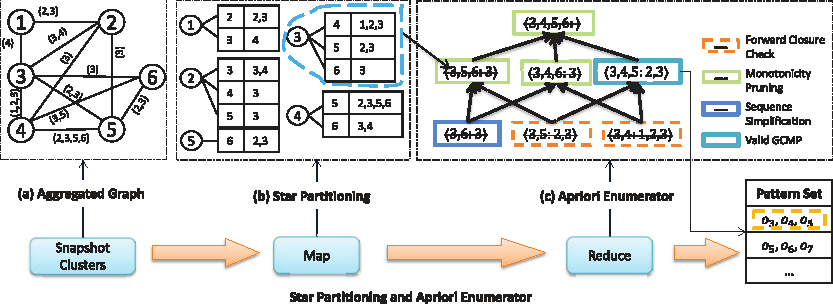
\includegraphics[width=\textwidth]{res/fig/sec-2/GCMPWorkFlow.pdf}
    \caption{Fasi di SPARE: \cite{DBLP:journals/pvldb/FanZWT16}}%
    \label{fig:chap-2:spare-workflow}
\end{figure}





\subsection{Snapshot Clusters}\label{subsec:gcmp-clustering}
La prima fase di SPARE è la generazione degli Snapshot.
Durante questo passo viene valutata la dimensione spaziale delle traiettorie in relazione alla dimensione temporale.
Scopo della fase è individuare ad ogni istante quali oggetti sono vicini e quali no, in modo da creare una sequenza di cluster che descrivono l'evolvere dei gruppi nel tempo.

Unico passo di preprocessing necessario prima di questa fase è la definizione di una scala temporale univoca all'interno del dataset.
Tutti i punti devono infatti essere rapportati a una scala di tempo omogenea, altrimenti i passi successivi non sarebbero possibili.
Il primo passo consiste quindi nella definizione di una sequenza di istanti univoci chiamata \(T_{db}\).
Tutti i punti di ogni traiettoria saranno espressi rispetto a questa scala.

Una volta determinata la scala temporale, si scompone ogni traiettoria nei suoi singoli punti.
Questi punti vengono poi raggruppati sulla base dell'istante temporale in cui accadono.
Per ogni istante temporale nella scala sarà determinato un insieme di punti che indicano la posizione delle rispettive traiettorie al tempo \(t_{i} \in T_{db}\).

A questo punto è necessario valutare quali punti siano vicini e quali no.
Come detto nella \cref{sec:comovement-definition}, algoritmi di clustering diversi generano pattern di movimento diversi (density o distance based).
SPARE supporta la ricerca di entrambi i pattern: sta all'utente scegliere quale algoritmo impiegare.
Questa scelta risulta trasparente alle successive fasi di itemset mining.

Questo è l'unico passo dove vengono considerate le dimensioni spaziali.
Intuitivamente, ogni traiettoria avrà al massimo una posizione per ogni istante temporale.
Il processo di clustering risulterà quindi partizionante, così da prevenire eventuali ambiguità nelle fasi successive.

Questa operazione produce una serie di raggruppamenti di cluster.
Uno snapshot \(S_t\) non è altro che una coppia \(\langle t, S(t) \rangle\) dove \(t\) rappresenta un instante temporale e \(S(t)\) l'insieme dei cluster individuati a quello specifico istante.

Gli snapshot sono l'output di questa prima fase.

\subsection{Star partitioning}\label{subsec:gcmp-star-partitioning}
Scopo di questa seconda fase è trasformare gli snapshot in itemset di due elementi che verranno poi processati nella fase successiva.
Durante la fase di star partitioning vengono aggregati gli snapshot generati nella fase precedente in maniera tale da avere per ogni coppia di oggetti l'insieme degli istanti temporali in cui hanno viaggiato vicini.
Successivamente per ciascun oggetto si valuterà in maniera univoca tutte le possibili combinazioni tra questo e gli altri oggetti, generando così un insieme di coppie, o itemset \(2\)-dimensionali, collegate alla sequenza di istanti in cui questi risultano vicini.

Dato uno snapshot \(S_{t}\) questo può essere rappresentato con un grafo non direzionato \(G_t\).
Tale grafico avrà nei nodi gli identificatori degli oggetti, tra nodi sarà presente un arco se quei due oggetti appartengono allo stesso cluster al tempo \(t\).
È possibile definire \(G_t\) per ogni snapshot \(S_t\).

Il singolo grafo tuttavia è poco espressivo, contiene infatti i dati relativi solo a un singolo istante temporale.
Si definisce quindi \(G_A\) o grafo aggregato una struttura composta dai singolo \(G_t\) e che descrive l'evoluzione dei cluster nel tempo.
\(G_A\) contiene gli stessi nodi di ogni \(G_t\).
Gli archi invece sono formulati nel seguente modo: esiste un arco tra due nodi se, all'interno di tutti i cluster presenti in tutti gli snaphot individuati, questi elementi compaiono assieme in almeno un cluster.
Oltre a questo sull'arco viene salvata la sequenza di istanti in cui i due oggetti compaiono nello stesso cluster.

Questo grafo così creato viene poi diviso in partizioni.
Per fare ciò si utilizza una struttura a stella, opportunamente modificata per evitare potenziali ripetizioni di coppie di nodi.
I nodi, o vertici, vengono infatti numerati sulla base di un ordinamento globale.
Una struttura così definita viene chiamata \textit{directed star}, o stella diretta (\cref{definition:directed-star})

\begin{definition}[Stella diretta]\label{definition:directed-star}

Dato un vertice con ID globale \(s\) si definisce una stella diretta \(Sr_s\) l'insieme dei vertici direttamente raggiungibili, o vicinato, 
aventi ID globale \(t > s\), definito \(s\) come ID della stella.

\end{definition}

\(G_A\) viene diviso in \(n\) stelle dirette, dove \(n\) è il numero di nodi nel sistema.
Grazie all'ordine globale dei vertici, ogni arco è contenuto in una sola partizione del grafo iniziale.
Ogni stella viene poi processata in maniera autonoma dalla fase di Apriori Enumeration

Questa operazione ha però un limite, ovvero il criterio di ordinamento.
Un criterio di ordinamento poco efficace porta a generare stelle sbilanciate.
Stelle con pochi archi terminano presto la computazione, mentre il sistema deve attendere che anche le stelle più grandi finiscano di essere computate.
Occorre quindi utilizzare un criterio di ordinamento efficace.

Dati \(n\) nodi, sono possibili \(n!\) ordinamenti.
Euristicamente si dimostra che un ordinamento basato sull'identificatore dei nodi porta a una suddivisione abbastanza bilanciata, di conseguenza SPARE non introduce nessun criterio di ordinamento particolare.

\subsection{Apriori enumerator}\label{subsec:gcmp-apriori}
Ultimo passo dell'algoritmo: date in ingresso le varie stelle dirette prodotte al passo precedente, produce gruppi di movimento come itemset.
Intuitivamente questa fase riconosce tra le stelle della fase precedente quali coppie di nodi possono essere considerate come valide.
Una coppia di nodi sarà valida se la sequenza collegate risulterà significativa rispetto a \(k\), \(l\) e \(g\).
Tutte le coppie valide saranno poi fuse in itemset, intersecando ogni volta le sequenze temporali e assicurandosi che ad ogni passo l'intersezione rimanga valida.
Questo processo di esplorazione produce itemset massimali aventi dimensione maggiore di \(m\).

Passando poi al procedimento, si parte dalle stelle generate alla fine della fase precedente.
Ogni stella viene scomposta in coppie nella forma \(\langle(o_v, o_n):(t_1, \ldots, t_n)\rangle\).
\(o_v\) è il vertice della stella, \(o_n\) è uno dei nodi della stella, \((t_1, \ldots, t_n)\) sono gli istanti temporali sull'arco \((o_v, o_n)\).

Eseguendo una generazione e ricerca di itemset, si può pensare di applicare l'algoritmo Apriori (\cref{subsec:apriori}).
Tuttavia non è possibile applicare questo algoritmo.
Il principio della monotonicità tra un set e un suo superset non è valido nel caso degli itemset individuati da SPARE.

Si supponga di considerare due candidati \(C_1 = \langle(o_1, o_2): 1,2,3,6\rangle\) e \(C_2 = \langle(o_1, o_3): 1,2,3,7\rangle\).
Fissati \(m = 2, k = 3, l = 2, g = 1\), né \(C_1\) né \(C_2\) risultano itemset validi, violano infatti sia il vincolo su \(l\) che su \(g\).
In \(C_1,\; maxgap = (6-3) > g\) mentre per \(C2, \; maxgap = (7-3) > g\).
Per quanto riguarda \(l\) invece \(C_1 = \{C_1' = \langle(o_1, o_2): 1,2,3\rangle, C_1'' = \langle(o_1, o_2):6\rangle\}\), risulta evidente che \(|C_1''| < l\).
Altrettanto vale per \(C_2 = \{C_2' = \langle(o_1, o_3): 1,2,3\rangle, C_2'' = \langle(o_1, o_3):7\rangle\}\), anche qui \(|C_2''| < l\).
Definito \( C_3 = C_1 \cup C_2 = \langle(o_1, o_2, o_3): 1,2,3\rangle\), questo itemset risulta valido rispetto a tutti e quattro i parametri.
\(C_3\) quindi è un superset valido di due set non validi: ciò viola la definizione classica di monotonicità.

Occorre quindi definire una nuova nozione di monotonicità.
Per giungere a questo obbiettivo sono necessari tre nuovi concetti: \textit{Maximal G-Connected sequence}, \textit{Decomposable sequence} e infine \textit{Sequence semplification}.

Data una sequenza di istanti temporali \(T\), la massima sequenza connessa rispetto a \(g\) (MGS) è la più lunga sotto-sequenza \(T'\) tale che non \(T'\) risulti connessa rispetto a \(g\) e non esista \(T'' \supset T' \) che sia a sua volta connessa rispetto a \(g\).
Ogni MGS deve essere quindi connessa rispetto a \(g\) e massima nel numero di elementi.
Ogni sequenza può essere divisa in \(n\) MGS.
Ciascuna di queste MGS è disgiunta dalle altre se non per il primo o l'ultimo elemento.
Inoltre l'unione di tutte le MGS produce la sequenza originale.
Infine ogni MGS di una sotto-sequenza può essere considerata come sotto-sequenza di una MGS della sequenza originale.
Prese ad esempio le sequenze \(T' = (1,2,4,5,6,9,10,11,13)~\text{e}~T'' = (1,2,4,5,6)\) con \(g = 2\).
\(T'\) ha due MGS: \(T'_a = (1,2,4,5,6)\) e \(T'_b = (9,10,11,13)\).
\(T''\) ha una sola MGS corrispondente alla sequenza stessa.
\(T''\) è sotto-sequenza di \(T'\), quindi ogni MGS di \(T''\) dovrà essere sotto-sequenza di una MGS di \(T'\).
In questo caso, \(T''\) e \(T'_a\) coincidono, dimostrando la validità della proprietà.

Una volta definito il concetto di MGS, si può introdurre quello di sequenza decomponibile (\textit{Decomposable sequence}).
Una sequenza decomponibile è una sequenza che ha al suo interno almeno una sotto-sequenza valida rispetto a \(k\), \(l\) e \(g\).
Una sequenza si definisce decomponibile se, presa una qualunque delle sue MGS, questa risulta consecutiva rispetto a \(l\) e avente lunghezza maggiore o uguale a \(k\).
Prese ad esempio la sequenza \(T' = (1,2,4,5,6,9,10,11,13)\) con \(k=5\), \(l=2\) e \(g = 2\), si considerano le due MGS \(T'_a = (1,2,4,5,6)\) e \(T'_b = (9,10,11,13)\).
\(T'_a\) risulta sia consecutiva rispetto a \(l\) che lunga \(k\) elementi, di conseguenza \(T'\) può essere definito come sequenza decomponibile.

Infine si definisce semplificazione di sequenza (\textit{Sequence simplification}).
Data un sequenza \(T\) si definisce sequenza semplificata o \(Sim(T)\) la sotto-sequenza di \(T\) ottenuta applicando due trasformazioni:

\begin{itemize}
    \item \textbf{f-step}. Rimuove i segmenti di \(T\) che non rispettano la consecutività rispetto a \(l\).
    \item \textbf{g-step}. Tra le MGS individuate sul risultato di f-step, scarta quelle che hanno dimensione minore di \(k\). 
\end{itemize}

Ad esempio dato \(T = (1,2,4,5,6,9,10,11,13)\) e \(l = 2, k = 3, g = 2\).
Alla fine di f-step \(T = (1,2,4,5,6,9,10,11)\), \(13\) viene scartato in quanto facente parte di una sotto-sequenza di lunghezza uno. 
Questa nuova sequenza ha due MGS: \((1,2,4,5,6)\) e \((9,10,11)\).
Il secondo di questi due elementi viene scartato in quanto avente dimensioni minori di \(k\).
La sequenza semplificata risulta quindi \((1,2,4,5,6)\).

Il processo di semplificazione di una sequenza può portare alla creazione di una sequenza nulla, qualora non siano verificate certe condizioni su \(l\) e \(k\).
Per definizione, la sequenza vuota non risulta decomponibile.
Alla luce di ciò è possibile esprimere la seguente proprietà: 
per qualunque \(T\) supeset di una sequenza decomponibile vale che \(Sim(T) \neq \varnothing\).
Banalmente, per una sequenza decomponibile è impossibile che  \(Sim(T) \neq \varnothing\), ciò vale anche per ogni suo superset.

Una volta introdotto quest'ultimo concetto è possibile formulare la nuova definizione di monotonicità (\cref{definition:monotonicity}):

\begin{definition}[Monotonicità]\label{definition:monotonicity}

Dato un candidato pattern \(P = \langle O:T \rangle\), se \(Sim(P.T) = \varnothing\) allora ogni pattern \(P'\) tale che \(P' \supseteq P\) può essere scartato.

\end{definition}

La definizione si basa sulla considerazione che qualunque superset di \(P\) è composto dall'unione degli oggetti e dall'intersezione delle sequenze temporali.
Risulta a questo punto scontato affermare che qualunque sotto-sequenza di una sequenza tale che \(Sim(T) \neq \varnothing\) a sua volta produce una sequenza vuota durante il processo di semplificazione.

Definita la nuova monotonicità, lo pseudocodice della fasi di Apriori Enumerator è presentato nel \cref{alg:apriori-enumerator}.

\begin{algorithm}[H]
\caption{\( Apriori Enumerator\)}\label{alg:apriori-enumerator}
\begin{algorithmic}[1]
\Require \(Sr_s\)
\State \(C \gets \varnothing\)
\ForEach{ archi \(c = <o_i \cup o_j, T_i \cap T_j> \) in \(Sr_s\)} \Comment{Per ogni 2-itemset.}
        \If{\(Sim(T_i \cap T_j) \neq \varnothing\)} \Comment{Se la semplificazione dell'intersezione delle sequenze risulta valida}
            \State \(C \gets C \cup c\) \Comment{La tupla viene aggiunta a C} 
        \EndIf
    \EndFor
\State \(level \gets 2\)  

\While{\(C \neq \varnothing\)} 
    \ForEach{\(c_1 \in C\)}
        \ForEach{\(c_2 \in C \land |c_1.O \cup c_2.O| = level\)} \Comment{Per tutti i validi n-itemset}
            \State \(c' = <c_1.O \cup c_2.O, c_1.T \cap c_2.T>\) \Comment{Vengono generati tutti gli n+1 itemset}
                 \If{\( Sim(c_1.T \cap c_2.T) \neq \varnothing \)} \Comment{Se la semplificazione dell'intersezione delle sequenze risulta valida}
                    \State \(C \gets C \cup c\) \Comment{La tupla viene aggiunta a C} 
                \EndIf
        \EndFor
        \If{Nessun c' viene aggiunto a \(C\) e \(c_1\) è un pattern valido} 
            \State \Return \(c_1\) \Comment{\(c_1\) viene restituito in output in quanto massimale} 
        \EndIf
    \EndFor
    \State \(O_u \gets \) unione di tutti i \(c.O\) in \(C\)
    \State \(T_u \gets \) unione di tutti i \(c.T\) in \(C\)
    \If{\(Sim(T_u) \neq \varnothing\)} \Comment{Controllo della forward closure} 
            \State \Return \(<O_u, T_u>\) \Comment{L'intersezione tra tutti i possibili itemset in C è massimale, quindi l'esplorazione è terminata} 
        \EndIf
\EndWhile

\end{algorithmic}
\end{algorithm}

SPARE parte dalla valutazione degli itemset contenenti due elementi.
Questi vengono filtrati secondo il principio di monotonicità descritto sopra.

Successivamente comincia l'esplorazione dello spazio di ricerca: ogni itemset valido \(n\)-dimensionale viene fuso con tutti gli altri tali da formare 
itemset \(n+1\)-dimensionali.
Questi sono poi valutati con la stessa logica usata sopra: i validi vengono mantenuti, gli altri sono scartati.
Nel caso un itemset durante questa fase non produca nessun superset valido, questo viene valutato come output.
Se risulta rilevante rispetto a \(m\) e \(k\) viene aggiunto all'output, altrimenti viene scartato.

Una volta terminato di computare i candidati del livello successivo, viene eseguito un controllo sulla \(forward closure\).
Questa operazione consiste nel fondere assieme tutti gli itemset da valutare e testare se il candidato così costruito sia un itemset valido e rilevante.
Se ciò risulta vero, allora questo può essere restituito in output in quanto massimale, altrimenti i candidati singoli sono valutati con la stessa logica descritta sopra.




  \chapter{L'algoritmo CU.TE}\label{chapter:chapter3}
  In questo capitolo verrà discusso dell'algoritmo C.U.T.E e
del contributo apportato da questo nuovo approccio nell'ambito del \textit{clustering} dei dati di traiettoria.

In primo luogo verrà definito il problema del \textit{Colossal Trajectory Mining},
successivamente saranno presentate l'idea e la realizzazione dell'algoritmo C.U.T.E,
infine saranno formulate alcune considerazione sui punti di forza e limiti di questo nuovo approccio.


\section{Idea generale}\label{sec:cute:idea}
\textit{Cu.Te}, o ClUstering TrajectoriEs, è un algoritmo di clustering overlapping il cui obbiettivo è l'analisi
di gruppi di oggetti in movimento. Questa ricerca viene condotta considerando sia la dimensione spazio-temporale
delle traiettorie sia eventuali dimensioni semantiche (come ad esempio, le municipalità di una città).

Lo scenario reale per la realizzazione di questo algoritmo è stata l'analisi condotta su
un insieme di traiettorie generate a Milano. All'interno di questo studio, i pattern di movimento sono
stati analizzati a diversi livelli.
Una prima analisi è stata condotta dividendo la superfice della città in piccole celle:questa ricerca
ha rivelato i pattern di movimento del traffico, individuando quali potessero essere le strade
maggiormente frequentate.
Succesivamente è stato realizzato uno studio basato sul vicinato: questo ha individuato i flussi di spostamento per specifiche categorie di utenti.
Infine una ricerca basata sulle municipalità ha mostrato quali fossero le aree della città più visitate da differenti gruppi di individui.

Lo scopo di \textit{Cu.Te} è dunque di estrarre i pattern di movimento che avvengono con una certa soglia di frequenza.

L'algoritmo \textit{Cu.Te} è etichettabile come algoritmo di \textit{colossal trajectory mining}.
L'idea alla base del \textit{colossal trajectory mining},
o mining di traiettorie su larga scala, interseca entrambi gli ambiti del clustering di traiettorie
e del colossal itemset mining (~\cref{subsec:problem:cim}).
La prospettiva del mining di itemset ad alta dimensionalità può essere impiegata anche nell'analisi di dati di traiettoria. Considerando la superfice
spazio-temporale coperta dall'insieme delle traiettorie e il numero di queste ultime, nella maggior parte dei casi risulterà evidente
che la dimensionalità di quest'ultimo dato sarà maggiore del precedente.
Risulta quindi possibile applicare algoritmi di mining di itemset su larga scala a dati di traiettoria.
In letteratura è possibile trovare riferimenti ad algoritmi di \textit{colossal itemset mining}~\cite{DBLP:journals/bdr/ApilettiBCGPM17, DBLP:conf/kdd/PanCTYZ03}
, tuttavia nessuno di questi è adatto alla ricerca di pattern di movimento, anche per la mancanza di
criteri di pruning basati sulle dimensioni spazio-temporali. Nonostante quindi la letteratura non
presenti una soluzione adatta, le idee alla base del \textit{colossal itemset mining} risultano sicuramente interessanti.

Parlando poi di clustering di traiettorie, rispetto a quanto trattato nella nella~\cref{sec:problem:trajectoryclustering}, è possibile aggiungere un'ulteriore divisione:
si definisce il clustering partizionante se ogni punto appartiene a un solo cluster, sovrapposto in caso contrario.
Applicando questo principio di classificazione agli algoritmi basati su traiettorie, gli algoritmi partizionanti considereranno la traiettoria nella sua interezza,
assegnandola quindi ad un solo cluster. Questa tipologia di clustering comporta però la perdita di informazioni tra i diversi cluster:
nonostante una traiettoria sia raggruppata in un cluster che massimizza la similarità tra i propri elementi,
questa può comunque condividere pattern interessanti con altre traiettorie appartenenti a cluster differenti.

Per superare il problema descritto sopra, gli algoritmi di clustering sovrapposto effettuano una divisione di ogni traiettoria
in sotto-traiettorie e effettuano un clustering partizionante su queste sotto-traiettorie.
Questa soluzione permette di conservare le relazioni intra-cluster, tuttavia una frammentazione troppo fine può causare
la perdita di \textit{rare pattern}, ad esempio eventi significanti che accadono con una bassa frequenza~\cite{DBLP:journals/tkdd/KohR16, DBLP:journals/geoinformatica/HuangPX06}.

Come già detto nella~\cref{sec:problem:trajectoryclustering}, il clustering classico non esprime vincoli temporali o ulteriori parametri adatti alla ricerca di traiettorie.
Per aggiungere la possibilità di esprimere vincoli sul tempo, sono stati introdotto i \textit{co-movement} patterns descritti nella~\cref{sec:problem:comovements-pattern}; algoritmi come \textit{G.C.M.P},
(~\cref{chapter:chapter2}), \textit{GeT Move}~\cite{DBLP:journals/ijitdm/PhanPT16} e  implementa la ricerca di questi pattern mischiando l'approccio basato su \textit{frequent itemset mining} e il clustering.
Entrambi questi framework discretizzano il tempo in bucket di dimensione finita, su cui poi applicano un clustering basato sulla densità, infine
ricercano pattern di movimento fondendo i vari cluster ottenuti nei differenti istanti temporali.

Rispetto a quanto presentato fin d'ora, \textit{Cu.Te} presenta le seguenti caratteristiche:

\begin{itemize}

  \item Flessibilità nell'impiego di dimensioni: all'interno di \textit{Cu.Te} è possibile aggiungere
  dimensioni personalizzate su cui condurre la ricerca, ad esempio si può espandere la dimensione spazio
  temporale aggiunendo il concetto di municipalità.
  Inoltre sono supportate dimensioni non esclusivamente monotone, come ad esempio i giorni della settimana.

  \item Continuità nello spazio tempo: nella ricerca di \textit{comomvement pattern} è possibile specificare vincoli di contiuità non solo sul tempo, ma anche sullo spazio.

  \item Efficienza nel pruning spazio-temporale: la strategia di pruning impiegata permette di ridurre
  lo spazio di ricerca dell'algoritmo sulla base della natura spazio-temporale delle traiettorie.

  \item Efficacia rispetto a problemi reali: \textit{Cu.Te} mette a disposizione una soluzione distribuita per il problema del \textit{Colossal Trajectory Mining}
  compatibile con dataset costruiti su problemi del mondo reale.
\end{itemize}


L'algoritmo segue tre step per la formazione dei cluster, come anche rappresentato in~\cref{fig:chap-3:cute-overview}

  \begin{figure}
    \centering
    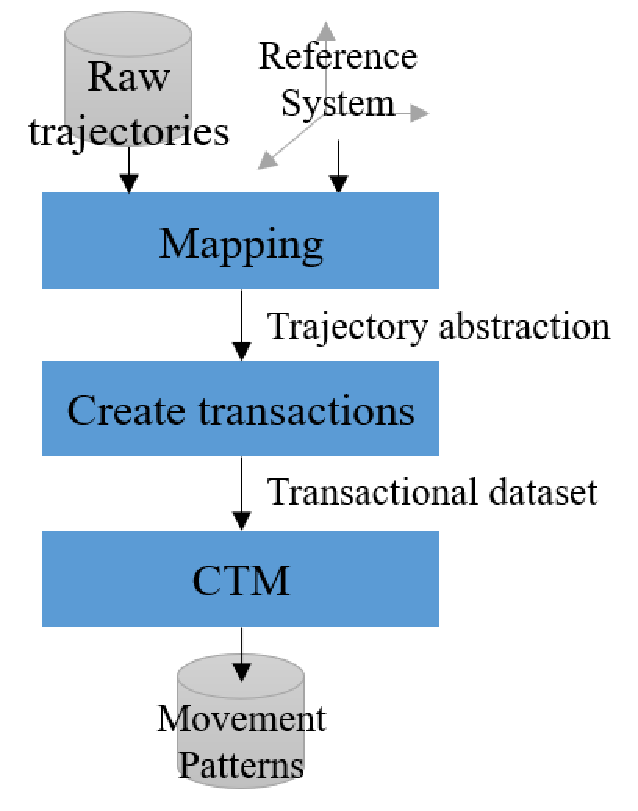
\includegraphics{/sec-3/cute-algorithm-overview.pdf}
    \caption{Rappresentazione grafica delle tre fasi dell'algoritmo Cu.Te,Fonte:~\url{https://which.souce?}}%
    \label{fig:chap-3:cute-overview}
  \end{figure}

  \begin{enumerate}
    \item \textbf{Mapping delle traiettorie:}

    In questo primo passo vengono analizzate le traiettorie presenti nel dataset. Da queste viene determinata la regione spazio-temporale
    in cui tutti gli oggetti si sono mossi. Successivamente l'area di movimento viene divisa in un insieme di celle omogenee per dimensioni nello spazio e nel tempo.
    A questo punto ad ogni traiettoria viene assegnato un insieme di celle secondo il seguente principio: una cella è attribuita ad una traiettoria quando quest'ultima ha
    almeno un punto che ricade entro i confini spazio-temporali della cella.

    \item  \textbf{Creazione delle transazioni:}

    Durante questa fase vengono poste le basi per l'\textit{itemset mining}: scopo di questa parte dell'algoritmo
    è infatti andare a generare l'insieme delle transazioni su cui verrà eseguita la ricerca di pattern.
    Ciò avviene considerando l'ouput della fase precedente e ribaltando la relazione cella traiettoria:
    mentre prima le traiettorie venivano condiderate in termini di celle percorse, ora si considera ogni cella in relazione alle traiettorie che almeno per
    un istante transitano al suo interno.

    \item \textbf{Colossal Trajectory Mining:}

    Ultima e più importante passaggio dell'algoritmo, produce in uscita i pattern di movimento.
    Dato l'output della fase precedente, ovvero un insieme di transazioni appositamemte creato,
    esegue una ricerca di itemset su dati ad alta dimensionalità.

  \end{enumerate}







\subsection{Definizione del problema}\label{subsec:cute:parameters}
Prima di concentrarsi sui singoli passi di \textit{Cu.Te}, occorre definire la formulazione dell'algoritmo.
Innanzitutto si pone necessario riprendere i concetti di itemset, supporto e transazione descritti nella~\cref{sec:problem:frequent-itemset-mining}
e di traiettoria grezza e astrazione di traiettoria presentati nella~\cref{subsec:problem:trajectorydata}.

A queste definizioni va aggiunto il concetto di sistema di riferimento: si definisce un sistema di riferimento un insieme di
quanti completo e continuo all'interno di una regione spazio-temporale.
I sistemi di riferimento sono fondamentali nel determinare le dimensioni spazio-temporali dei punti delle varie traiettorie,
un esempio su tutti può essere una scala di riferimento espressa in coordinate polari.
Tuttavia è possibile definire anche sistemi di riferimento che utilizzano metriche diverse dalle coordinate sopracitate,
ottenendo così diversi effetti sulla rappresentazione dei dati.

Per quanto riguarda invece l'aspetto collegato alla ricerca di itemset,
in \textit{Cu.Te} viene introdotto il concetto di \textit{Cohesion} o coesione: dato un itemset \textit{I} = \{ \textit{i\textsubscript{1}},\ldots, \textit{i\textsubscript{n}}\}
avente supporto definito come \textit{s}, si definisca la funzione \textit{allTransaction(i)} %chktex 36
 che dato un item \textit{i} restituisce l'insieme delle
transazioni che lo supportano. A questo punto è possibile definire la coesione con la seguente formulazione:

\[ coh(I) = \frac{\lvert \lvert allTransaction(\textit{i\textsubscript{1}})~\cap ,\ldots, \cap~allTransaction(\textit{i\textsubscript{n}}) \rvert\rvert}{\lvert \lvert allTransaction(\textit{i\textsubscript{1}})~\cup ,\ldots, \cup~allTransaction(\textit{i\textsubscript{n}}) \rvert\rvert} \]

Considerando che il numeratore corrisponde esattamente a \textit{s}, allora è possibile esprimere l'equazione come:

\[ coh(I) = \frac{s}{\lvert \lvert allTransaction(\textit{i\textsubscript{1}})~\cup ,\ldots, \cup~allTransaction(\textit{i\textsubscript{n}}) \rvert\rvert} \]

La nuova misura permette di misurare la compattezza di un itemset rispetto agli elementi che lo compongono.
La coesione si pone quindi come meccanica di filtraggio aggiuntiva al supporto:
mentre quest'ultimo è una misura in termini assoluti di frequenza, la coesione risulta una metrica relativa alla frequenza dei singoli elementi.
Ne segue che un alto valore di coesione andrà a scartare quegli itemset i cui item risultano molto sparsi all'interno delle transazioni,
mantenendo invece quelli che risultano più compatti.

Una volta definiti questi due concetti, è opportuno elencare e definire i parametri
utilizzati da \textit{Cu.Te}.

\begin{itemize}

  \item Quanto spaziale \textit{s}:
  Definisce la dimemsione spaziale del sistema di riferimento, in relazione alle coordinate polari di ogni punto.

  \item Quanto temporale \textit{t}:
  Definisce la dimensione temporale del sistema di riferimento rispetto al tempo misurato in secondi di ogni punto di una traiettoria.
  \item Soglia di distanza spaziale\(~\epsilon \):
  Dati due punti \textit{p\textsubscript{1}, p\textsubscript{2}} e una funzione di distanza spaziale \textit{d\textsubscript{s}},
  si definisce \(~\epsilon \) come la soglia sotto la quale due punti si considerano vicini.
  \item Soglia di distanza temporale\(~\tau \): analogamente a quanto detto sopra, il parametro \(~\tau \) permette di specificare
  una soglia massima per la distanza tra due punti nel tempo.
  \item Dimensione minima\(~\gamma \): Questo parametro riguarda il numero minimo di item all'interno di ogni itemset restituito in output alla fine dell'algoritmo.
  \item Supporto minimo\(~\alpha \): La frequenza minima oltre cui ogni itemset deve apparire all'interno dell'insieme delle transazioni.
  \item Coesione minima\(~\beta \): Come definito sopra, esprime un limite inferiore alla coesione degli itemset prodotti dall'algoritmo.

\end{itemize}

Grazie a questi parametri, risulta possibile per \textit{Cu.Te} affrontare il problema
della ricerca di \textit{comovement-pattern}, descritto nella \cref{sec:problem:comovements-pattern}.
Scendendo nel dettaglio, \(~\gamma \) esprime la dimensione minima di un gruppo considerato interessante, mentre
\(~\alpha \) il numero minimo di istanti spazio-temporali in cui tutti i membri del gruppo sono considerati vicini.
\(~\epsilon \) rappresenta il criterio di vicinanza spaziale tra due punti, \(~\tau \) invece permette la ricerca dei diversi pattern di movimento:
con \(~\tau \) = 1 si ha un vincolo stringente sulla continuità temporale, andando quindi a ricercare pattern \textit{flock},
dall'altra parte con un valore uguale a \(~\infty \), si rilassa al massimo la continuità temporale, ottenendo
così dei risultati classificabili come \textit{Swarm}. Infine con qualunque valore intermedio tra 1 e  \(~\infty \),
\textit{Cu.Te} esegue la ricerca di pattern \textit{Group} degeneri, ovvero con vincolo \textit{L} posto uguale a 1.




\subsection{Mapping del dataset}\label{subsec:cute:mappingdataset}
Inizialmente, il dataset delle traiettorie è composto da un insieme di punti aventi le seguenti caratteristiche:
una dimensione temporale espressa in secondi, due coordinate spaziali per determinare la sua posizione rispetto a un sistema di coordinate polari e
infine un identificatore di traiettoria. A queste dimensioni possono essere poi aggiunte altre informazioni, che non sono prese in considerazione durante l'esecuzione dell'algoritmo.

Scopo di questa prima fase di \textit{Cu.Te} è determinare un sistema di riferimento per i punti all'interno del dataset ed esprimere questi ultimi in
relazione al nuovo sistema.

Come indicato nella~\cref{subsec:cute:parameters}, è possibile determinare un sistema di riferimento che più aderisce alle esigenze del problema.
In questo caso la necessità principale in vista della fase di \textit{Colossal Trajectory Mining} è la ridotta dimensionalità dello spazio-tempo rispetto al numero di traiettorie
processate: si rende infatti necessario avere un numero di riferimenti spazio-temporali strettamente inferiorie alle traiettorie presenti nel database.

L'idea per risolvere questa esigenza è la divisione della superficie spazio-temporale in celle omogenee per range. Dato l'intero volume dello spazio-tempo
coperto dalle traiettorie nel dataset, questo viene partizionato in parallelepipedi di medesime dimensioni. Una cella \textit{c} è un parallepipedo, generato dal
partizionamento dello spazio-tempo coperto dalle traiettorie, avente un indice univoco.
Questa suddivisione costituisce quindi il nuovo sistema di riferimento del problema, è necessario quindi esprimere i punti all'interno del dataset rispetto a questo nuovo sistema.

Partendo dallo spazio, ogni punto di traiettoria, per definizione, determina la propria posizione sulla superficie terrestre utilizzando due coordinate, latitudine e longitudine.
Prendendo in considerazione l'area di un insieme di traiettorie, il processo per la generazione di celle spaziali è il seguente: per prima cosa si determina, mediante
il parametro \textit{s} la dimensione dei lati spaziali di una cella; successivamente si definisce la funzione \textit{pointToCell}, tale funzione ha il compito
di restituire, dato un punto, la cella di appartenenza. La cella in questione viene calcolata supponendo di scomporre la superficie terrestre in quadrati aventi lato \textit{s}
a partire da Null Island (punto avente latitudine e longituidne pari a zero)~\footnote{\url{https://blogs.loc.gov/maps/2016/04/the-geographical-oddity-of-null-island/}}.
In~\cref{fig:chap-3:milan-cell-division} è possibile vedere un esempio di divisione in celle applicato sulla città di Milano.

\begin{figure}
  \centering
  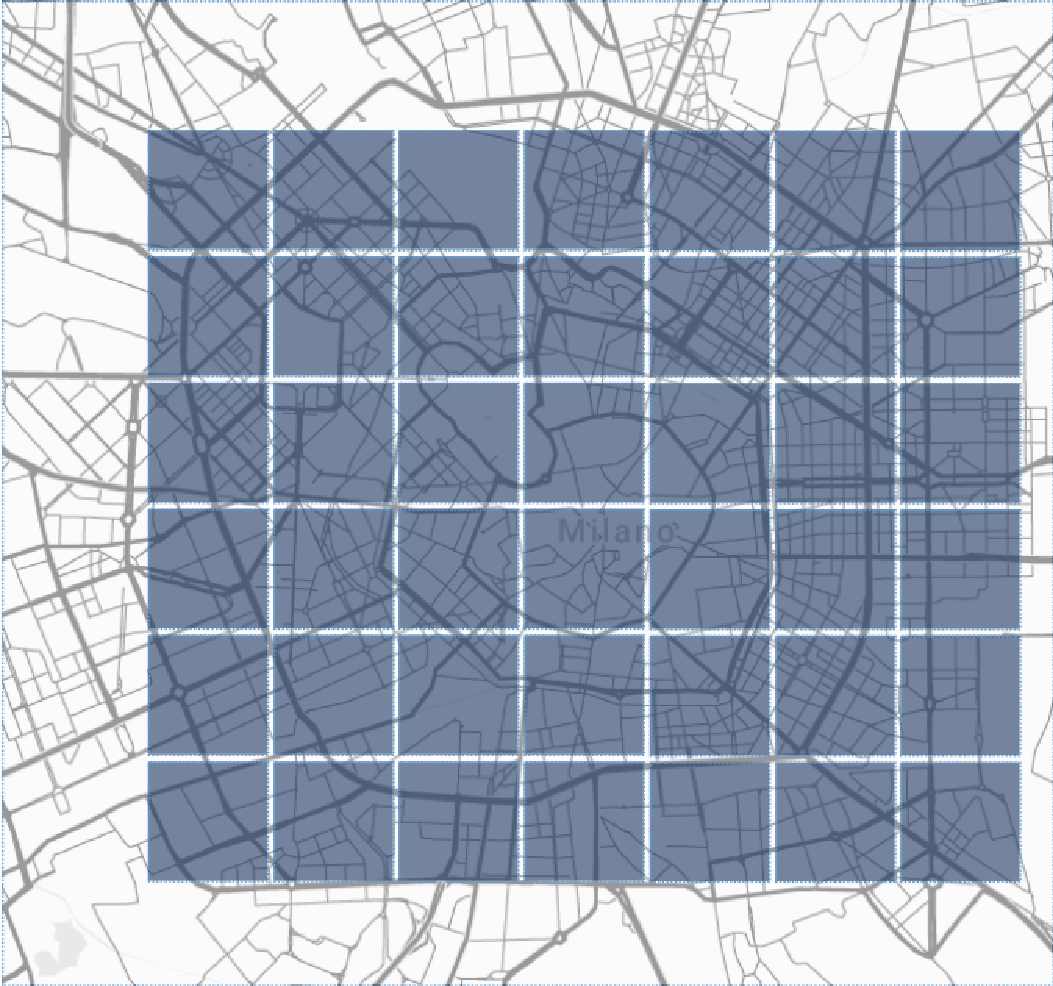
\includegraphics[scale=.6]{/sec-3/MilanCells.pdf}
  \caption{Suddivisione della città di Milano in celle,Fonte:~\url{https://which.souce?}}%
  \label{fig:chap-3:milan-cell-division}
\end{figure}

Per quanto riguarda la dimensione temporale invece, le possibilità a disposizione sono diverse, ma tra tutte si è scelto di supportare due principali scale: una basata sulle ore del giorno mentre l'altra sui giorni della settimana.
Rispetto a una metrica di tempo monotona basata su data e ora di ogni singolo punto, come ad esempio in \textit{G.C.M.P}, una scala circolare ha due vantaggi: il primo riguarda
il supporto a pattern ciclici che verrebbbero ignorati da una metrica monotona e in secondo luogo il ridotto range di valori della scala (da 0 a 23 in caso di scala giornaliera, da 0 a 6 in quella settimanale)
previene l'esplosione nel numero di celle al crescere del dataset.

Una volta determinata il lato spaziale delle celle e la durata temporale, processando le traiettorie nel dataset mediante una variazione della funzione \textit{pointToCell} adattata alla
gestione di celle tridimensionali, viene generato l'insieme delle celle \textit{C}. Questo set contiene tutte le celle, determinate dall'apposita funzione, tali che almeno
un punto di una traiettoria appartiene a quella cella. Questo approccio alla generazione delle celle garantisce che non vengano generate celle vuote, ovvero dove non passa nessuna traiettoria,
garantendo quindi una maggiore efficenza rispetto alla suddivisione assoluta della superficie spazio-temporale coperta dal dataset.

Ottenuto l'insieme delle celle, è necessario per concludere questa prima fase esprimere ogni traiettoria nel nuovo sistema di riferimento: così facendo una traiettoria non sarà più definita come
la composizione di diversi punti isolati nel tempo, ma come un'insieme di celle. La~\cref{fig:chap-3:trajectory-cell-division} mostra un esempio di conversione in un sistema di riferimento basato su celle:

\begin{figure}
  \centering
  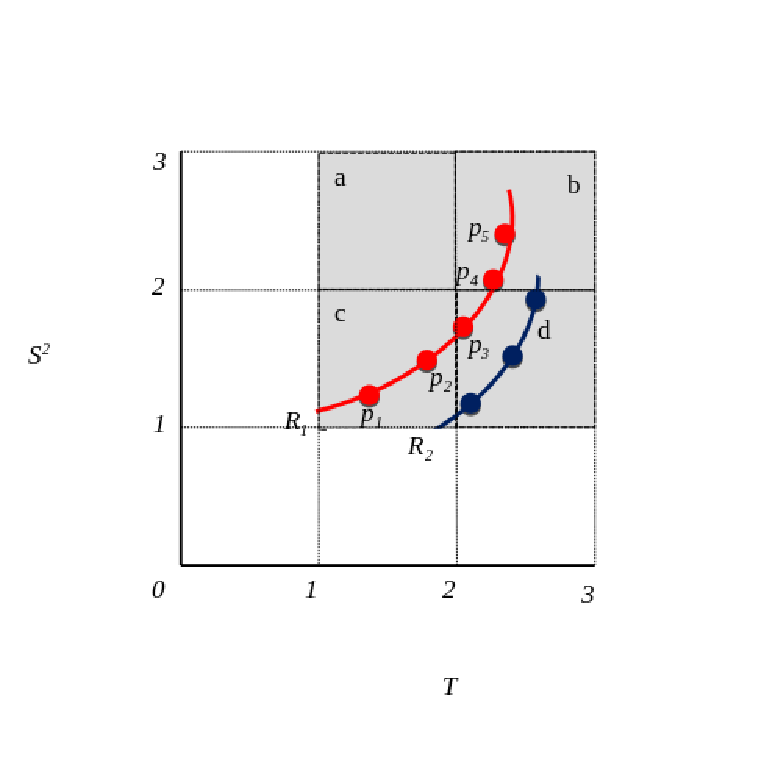
\includegraphics[scale=.8]{/sec-3/TrajectoryCellDecomposition.pdf}
  \caption{Mapping di due traiettorie, \textit{R\textsubscript{1}, R\textsubscript{2}} in un sistema di riferimento basato su celle.}%
  \label{fig:chap-3:trajectory-cell-division}
\end{figure}

Prendendo in considerazione le traiettorie \textit{R\textsubscript{1}, R\textsubscript{2}}, è possibile vedere come i punti \textit{p\textsubscript{1}, p\textsubscript{2}} appartengano alla cella \textit{c},
\textit{p\textsubscript{3}} a \textit{d} mentre \textit{p\textsubscript{4}, p\textsubscript{5}} a \textit{b}; analogamente ogni punto della traiettoria \textit{R\textsubscript{2}} sia attribuibile a \textit{d}.
Il set di celle del problema sarà quindi composto dalle seguenti celle: \textit{\textless b, c, d \textgreater} mentre le due traiettore saranno espresse in funzione del nuovo sistema di rifermimento come segue:

\begin{itemize}

  \item \textit{R\textsubscript{1}}: \{ \textit{b,c,d} \}
  \item \textit{R\textsubscript{2}}: \{ \textit{d} \}

\end{itemize}

Va sottolineato infine che, sebbene appaia nell'immagine, la cella \textit{a} non viene effettivamente generata, poiché nessuna traiettoria ha un punto entro i suoi confini.

Una volta che le traiettorie sono state espresse nelle nuove coordinate, questo primo passo dell'algoritmo giunge a termine.

Nonostante le operazioni eseguite in questa fase possano sembrare lineari, le basi che vengono gettate influenzano l'esecuzione dell'algoritmo e gli stessi risultati finali:
tra tutte, la scelta delle dimensioni di ogni cella influenza molto i passaggi successivi. Celle piccole produrranno traiettorie lunghe, estendendo il possibile spazio di ricerca di ogni cluster.
Tanto più amplio lo spazio di ricerca, tanto più a lungo dura la sua esplorazione, tuttavia è possibile eseguire una ricerca più fine su di esso.
Lati spaziali più ampli e dimensioni temporali ridotte generano celle più grandi, con uno spazio di ricerca più ridotto e risultati più grezzi.

Nonostante quanto affermato all'inizio, non è completamente corretto dire che tutti i dati che non siano collegati alla posizione nello spazio-tempo della traiettoria siano ignorati.
È infatti possibile considerare un numero variabile di dimensioni durante il processo di generazione delle celle. Tale aggiunta infatti non fa altro che andare ad aumentare la dimensionalità della singola cella,
ciò implica un numero maggiore di celle in cui dover convertire una traiettoria, ma il risultato finale della fase sarà il medesimo, l'unica differenza sarà nell'avere mediamente traiettorie
associate a un numero maggiore di celle.



\subsection{Creazione delle transazioni}\label{subsec:cute:transactioncreation}
Nella prima fase viene prodotto un dataset nella forma \textit{<t\textsubscript{i}, (c\textsubscript{1},\ldots,c\textsubscript{n})>},
dove \textit{t\textsubscript{i}} rappresenta l'id di una certa traiettoria, mentre \textit{c\textsubscript{1},\ldots,c\textsubscript{n}}
l'insieme di celle in cui tale percorso è stato convertito.
Questo dataset tuttavia non è ancora adatto ad essere sottoposto a mining, poiché in questa situazione l'insieme delle transazioni è composto dalle traiettorie,
mentre quello delle feature dalle celle.
Un'operazione di ricerca di regole associative va ad individuare tra le feature quelle che compaiono assieme con almeno una certa frequenza,
quindi in questo caso il risultato dell'algoritmo sarebbe varii raggruppamenti di celle.
Questi insiemi possono essere sicuramente utili ad individuare percorsi frequenti e trafficati, ma non sono in grado di descrivere gruppi di movimenti comuni ad un certo insieme di oggetti.

Scopo di questo secondo passo di \textit{Cu.te} è quindi modificare il dataset ottenuto dalla prima fase
in modo da renderlo valido per la ricerca di pattern di movimento.
Per realizzare questa trasformazione, occorre invertire il ruolo di celle e traiettorie all'interno del dataset: prendendo come
ipotesi di invertire la relazione tra traiettoria e insieme di celle che la compongono, si ottiene la versione trasposta del dataset originale.
La versione invertita del database sarà quindi composta dalle singole celle del problema che ora saranno identificate
come le transazioni, mentre il ruolo delle traiettorie sarà di feature. Così facendo ad ogni cella sarà associato l'insieme delle traiettorie di cui
fa parte.
In questa situazione la ricerca di itemset frequenti produce raggruppamenti di traiettorie che hanno una frequenza maggiore
a una certa soglia di supporto.
Tale soglia può essere interpretata come il numero minimo di celle, ovvero di istanti spazio-temporali, che
l'intero gruppo di traiettorie deve aver condivisio per essere considerato interessante.
Alla luce di questa interpreatzione, diviene chiaro che questo vincolo svolge la stessa identica funzione del parametro \textit{k} definito nella~\cref{sec:comovements-pattern},
per quanto riguarda invece \textit{m}, questo è espresso con  \(~\gamma \), presentato nella~\cref{subsec:cute:parameters}; infine \textit{g} è espresso come \(~\tau \) nella formalizzazione di \textit{Cu.Te}.

Invertendo il dataset è quindi possibile eseguire una ricerca di comovements pattern, ma l'inversione ha un'altra importante proprietà:
analizzando il rapporto tra il numero di celle generate nella prima fase e di traiettorie in tutto il dataset, è corretto affermare che
la quantità di queste ultime superi di gran lunga l'altra. La ricerca di pattern di movimento in città presenta infatti un'area spazio-temporale
ridotta rispetto agli oggetti che si muovono sopra questa superficie.
Di conseguenza il dataset che considera come transazioni le celle e come feature le traiettorie sarà etichettabile come dataset ad alta dimensionalità, adatto quindi a essere processato con le tecniche proprie del
\textit{Colossal Trajectory Mining}.




\subsection{Colossal Trajectory Mining}\label{subsec:cute:ctm}
Ultimo e più importante passaggio dell'algoritmo: dato il dataset prodotto in output dalla fase precedente,
viene eseguita una ricerca di pattern di co-movimento utilizzando i principi del \textit{Colossal Trajectory Mining}.




\section{Dettagli implementativi}\label{sec:implementation}

\section{Punti di forza e limiti}\label{sec:cute:strenght}




  \chapter{Test sperimentali}\label{chapter:chapter4}
  
In questo capitolo vengono presentati i risultati ottenuti dall'algoritmo CUTE. 
In primo luogo sono analizzati i dataset utilizzati nei test svolti.
Successivamente sono mostrati i risultati ottenuti da CUTE per quanto riguarda i cluster individuati e le performance in relazione al tempo.
Infine è discusso il confronto tra CUTE e SPARE: sono presentate le differenze tra gli approcci e i risultati ottenuti.

I test sono stati eseguiti su un cluster composto da 15 nodi, ognuno dei quali equipaggiato con un 8-core i7 CPU 3.60Hz e 32GB di RAM e interconnessi da una ethernet Gigabit.


\section{Dataset}\label{sec:comp:dataset}
Nel processo di testing e confronto tra i due algoritmi sono stati impiegati due diversi dataset.

Il primo dataset utilizzato è Geolife (\cite{GeolifeG31:online}).
Questo dataset è composto da un insieme di traiettorie raccolte in Asia, in particolare in prossimità della città di Pechino.
In Geolife sono presenti 17158 traiettorie distinte, composte da punti contenenti latitudine, longitudine e altitudine.
Il \(91\%\) delle traiettorie nel dataset sono generate da dispositivi aventi tempo di campionamento compreso tra \(1\) e \(5\) secondi.
Il tempo totale coperto da tutte le traiettorie nel dataset è circa quattro anni.

Il secondo dataset impiegato è composto da un insieme di traiettorie registrate nella città di Oldenburg.
Questo conta 1000000 traiettorie, a differenza di quanto detto prima, i punti non sono espressi in coordinate polari, ma in coordinate cartesiane rispetto a un sistema di riferimento custom.
Anche per quanto riguarda la dimensione temporale, il dataset viene fornito con punti aventi una componente temporale relativa a una sequenza di istanti.
La sequenza in questione conta 245 istanti distinti.

La \cref{tab:metrics-dataset} riassume le caratteristiche principali dei dataset impiegati nei test.
Per quanto riguarda il numero di traiettorie, Geolife viene utilizzato sempre nella sua interezza, Oldenburg invece partizionato diversamente a seconda delle situazioni di impiego.


\begin{table}[H]
    \centering
   \begin{tabular}{||c c c c c||}
 \hline
     Dataset & Spazio & Tempo & Punti & Traiettorie\\ [0.4ex] 
 \hline\hline
    Geolife & Coordinate polari & yyyy-mm-gg hh:mm:ss & 18891115 & 17158 \\ 
 \hline
     Oldenburg & Coordinate cartesiane & Sequenziale & 64895840 & 1000000 \\ 
 \hline
\end{tabular}
    \caption{Riassunto delle caratteristiche principali dei due dataset utilizzati}
    \label{tab:metrics-dataset}
\end{table}


\section{CUTE}\label{sec:comp:cute}
Di seguito sono presentati tutti i test eseguiti su CUTE.
Questi test sono stati condotti, salvo specificato diversamente, su un insieme di \(9\) executors, aventi ciascuno \(3\) cores.
Ad ogni executor sono stati assegnati \(12\) gigabyte di RAM.

\subsection{Cluster individuati}\label{subsec:comp:cluster}
Scopo dell'algoritmo CUTE è la ricerca di pattern di movimento aventi caratteristiche di rilevanza rispetto al percorso e dimensione del gruppo in movimento.
Essendo CUTE un framework generico, deve essere possibile distinguere le varie tipologie di pattern di movimento (swarm, flock, platoon) e verificare le variazioni nel numero degli itemset.
Intuitivamente, una ricerca di swarm produrrà molti più itemset validi di una di flock, per via dei vincoli più rilassati.
Allo stesso modo i diversi livelli di grana delle celle dovranno produrre risultati diversi a seconda delle soglie di supporto e dimensioni.
Per condurre questi test, il dataset utilizzato è stato Geolife, in quanto compatibile con le scale settimanale e giornaliera.

Primo e fondamentale ambito di testing è stato il sistema di riferimento e di conseguenza la granularità di ogni cella.
Questo parametro risulta particolarmente interessante: in un algoritmo di row enumeration, come CUTE o Carpenter, il numero di transazioni determina la complessità dell'algoritmo.
Come detto nella \cref{sec:cute:cim}, nel primo passo della ricerca dei gruppi, ogni cella corrisponde a una transazione.
A seconda del valore dei parametri \(s\) e \(t\), ovvero l'intervallo spaziale e quello temporale, il volume di ogni cella e il loro numero complessivo cambia.
Le \cref{fig:chap-4:cells} mostra il numero di celle al variare del lato \(s\) tra \(1,5,10\)KM.
All'aumentare del lato spaziale delle celle, la compressione dello spazio di ricerca aumenta, diminuendo quindi il numero di celle.
La \cref{fig:chap-4:cellt} mostra invece il rapporto tra \(t\) che varia su \(24h,7gg\) e in assenza di dimensione temporale e le celle. 
Com'è possibile vedere, il numero delle celle a parità di spazio non cresce esponenzialmente, ma di un fattore moltiplicativo collegato ai possibili valori dell'intervallo temporale.

\begin{figure}
  \centering
  \begin{subfigure}{.5\textwidth}
  \centering
   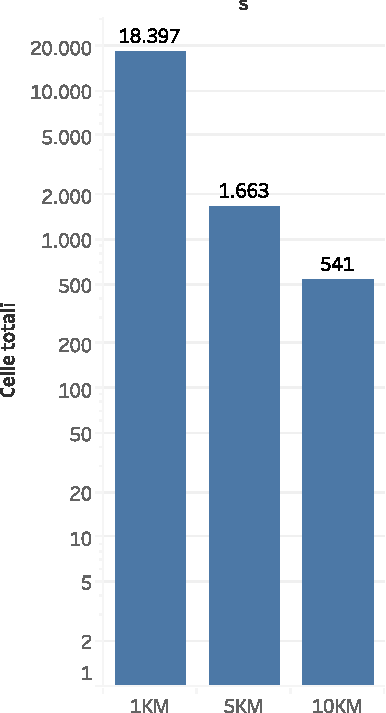
\includegraphics[scale=0.5]{res/fig/sec-4/Cells.pdf}
   \caption{\(s\) tra \(1,5,10\) KM}
  \label{fig:chap-4:cells}
\end{subfigure}%
\begin{subfigure}{.5\textwidth}
  \centering
   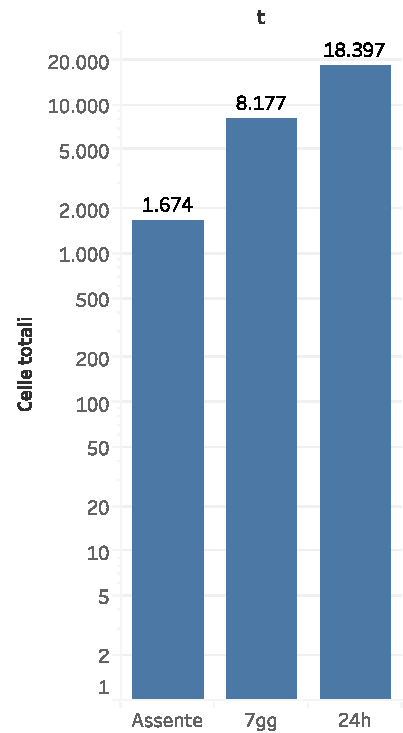
\includegraphics[scale=0.5]{res/fig/sec-4/CellT.pdf}
   \caption{\(t\) tra 24h, 7gg e assenza di tempo}
  \label{fig:chap-4:cellt}
\end{subfigure}%
  \caption{Celle alla variazione di \(s\) a sinistra, \(t\) a destra}%
  \label{fig:chap-4:cellst}
\end{figure}

Su ognuna delle configurazioni sopra espresse è stata eseguita una ricerca di itemset rispetto alle variazioni dei parametri in gioco presentati nella \cref{subsec:cute:params}.
I valori espressi per questi parametri sono riassunti nella \cref{tab:parameters-variation}.
Nei successivi test, dove non specificato, ai parametri è assegnato il valore di default (in grassetto nella \cref{tab:parameters-variation}).

\begin{table}[H]
    \centering
   \begin{tabular}{||c c c||}
 \hline
     Param. & Significato & Valori \\ [0.4ex] 
 \hline\hline
   s & Lato spaziale cella & \textbf{1KM}, 5KM, 10KM \\
   \hline
   t & Lato temporale cella & \textbf{24h}, 7gg, assenza di tempo \\
   \hline
   minsize & dimensione dei gruppi & 5, \textbf{10}, 15 \\
   \hline
   minsup & supporto minimo & 5, \textbf{10}, 15 \\
   \hline
   \(\epsilon\) & soglia spaziale & 2, \textbf{5}, 10, \(\infty\) \\
   \hline
   \(\tau\) & soglia temporale & 1, \textbf{2}, \(\infty\) \\
 \hline
\end{tabular}
    \caption{Parametri e il loro valore di default (in grassetto)}
    \label{tab:parameters-variation}
\end{table}

In particolare il focus di questi test è capire come varia il numero dei cluster individuati all'interno del problema.
I valori di supporto e dimensione minima coincidono e sono stati determinati empiricamente.
Il range di \(\epsilon\) varia tra \((2, 5, 10, \infty)\) mentre quello di \(\tau\) tra \((1, 2, \infty)\).
Mentre i valori di \(\epsilon\) sono stati scelti sperimentalmente, quelli di \(\tau\) sono stati selezionati sulla base del range delle scale temporali utilizzate.
In particolare le scale giornaliere e settimanale presentano una natura ciclica.
Una scala ciclica non ha un valore massimo assoluto e un minimo assoluto, ma prevede che il valore successivo al massimo sia il minimo.
Questa circolarità impatta la misura della distanza tra due punti.
Questa è definita come la dimensione del più piccolo intervallo tra due punti: può essere quindi la minima distanza calcolata dal maggiore al minore o viceversa.
Ciò comporta che all'interno di una scala ciclica, i valori siano molto più vicini rispetto a una monotona.
Quindi è molto facile che considerando valori alti di \(\tau\) il risultato tenda a essere quello di \(\tau = \infty\).
Ciò vale soprattutto per la scala settimanale: essendo solamente \(7\) i giorni della settimana e la scala ciclica per definizione, la distanza massima tra due qualunque elementi è al massimo \(3\).
Questo implica che l'unico valore plausibile per eseguire una ricerca di platoon su questa scala sia \(2\).
\(\tau\) determina inoltre la categoria di co-movement pattern individuato, ad esempio su scala settimanale vale che:
\begin{itemize}
    \item \(\tau = 1\): Flock
    \item \(\tau = 2\): Platoon g-connected
    \item \(\tau = \infty\): Swarm
\end{itemize}

\begin{figure}
  \centering
  \begin{subfigure}{.5\textwidth}
  \centering
   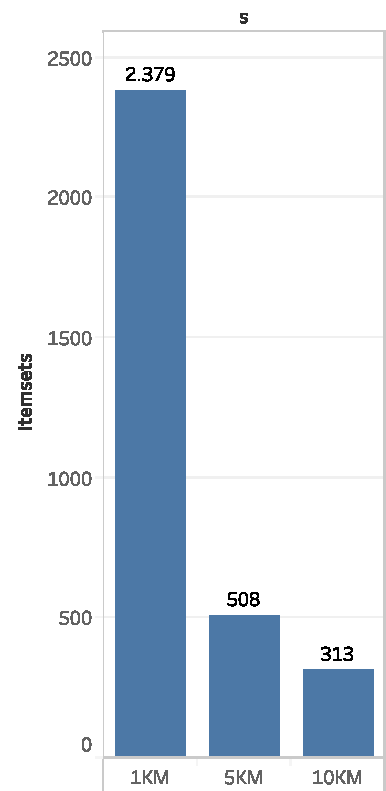
\includegraphics[scale=0.5]{res/fig/sec-4/itemset/ItemsetS.pdf}
   \caption{\(s\) tra \(1,5,10\) KM}
  \label{fig:chap-4:ItemsetS}
\end{subfigure}%
\begin{subfigure}{.5\textwidth}
  \centering
   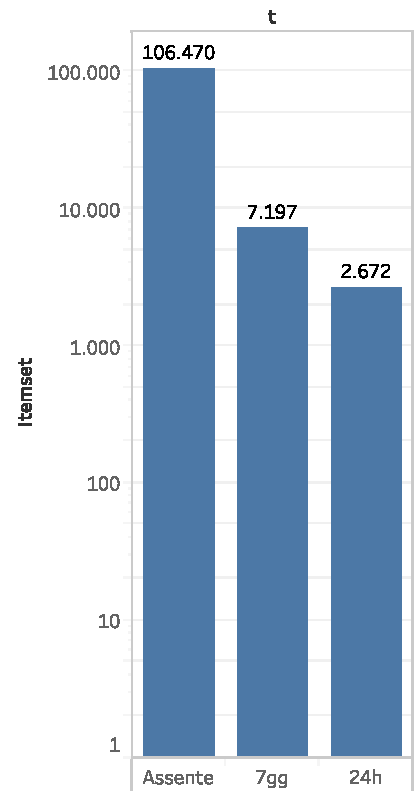
\includegraphics[scale=0.5]{res/fig/sec-4/itemset/ItemsetT.pdf}
   \caption{\(t\) tra 24h, 7gg e assenza di tempo}
  \label{fig:chap-4:ItemsetT}
\end{subfigure}%
  \caption{Numero di itemset alla variazione di \(s\) a sinistra, \(t\) a destra}%
  \label{fig:chap-4:ItemsetSandT}
\end{figure}

Le \cref{fig:chap-4:ItemsetS,fig:chap-4:ItemsetT} mostrano le variazioni del numero di itemset su \(s\) e \(t\).
Per quanto riguarda le variazioni nel lato spaziale delle celle \(s\), i risultati sono coerenti con quanto atteso: all'aumentare dell'area coperta dalle celle, calano il numero di itemset individuati (\cref{fig:chap-4:ItemsetS}).
Ciò è coerente con la natura del problema: se ogni cella corrisponde a una transazione, al calare del numero di transazioni a parità di supporto calano sia il numero di itemset frequenti che il tempo necessario per eseguire la ricerca.
Per \(t\), i risultati presentati sono stati ottenuti ponendo \(\tau = \infty\), questo perché non avrebbe avuto senso considerare la continuità nel tempo considerando una scala come l'assenza di tempo che esclude questa dimensione (\cref{fig:chap-4:ItemsetT}).
Alla luce di ciò, la dimensione temporale \(t\) presenta invece un trend opposto a \(s\) per quanto riguarda gli itemset individuati: l'impiego della scala giornaliera rispetto a quella settimanale individua meno itemset sia in caso di vincoli su \(\tau\) che in sua assenza.
L'assenza di una dimensione temporale invece produce risultati di circa un ordine di grandezza superiori rispetto agli altri due.
Questo fenomeno può essere direttamente collegato all'aumento del numero di celle a seguito dell'adozione di diverse scale temporali.
L'introduzione di una nuova dimensione produce infatti un'ulteriore suddivisione dello spazio di ricerca: un pattern valido in uno spazio \(n\)-dimensionale può non risultarlo più in uno \(n+1\) dimensionale, poiché il gruppo può non risultare vicino nella nuova dimensione.
Questa frammentazione sarà tanto più netta tanti più valori possibili avrà la scala della nuova dimensione.
Applicando quanto detto sopra alle scale temporali, l'assenza di tempo non produce nessuna ulteriore divisione, la scala settimanale e quella temporale aggiungono una cardinalità di rispettivamente \(7\) e \(24\) intervalli.
La frammentazione dello spazio di ricerca causa quindi la differenza nei risultati delle tre scale.


Le \cref{fig:chap-4:ItemsetMinsize,fig:chap-4:ItemsetMinsupp} individuano le variazioni di pattern riconosciuti al variare di supporto e dimensione minima.
Minsup e minsize (\(\alpha, \gamma\)) sono fatti variare tra \(5, 10, 15\).
Entrambi i parametri si comportano come atteso: all'aumentare del valore cala il numero di itemset individuati.
La ricerca di gruppi di dimensioni maggiori o che abbiano un elevato tempo di viaggio riduce il numero di itemset validi.

\begin{figure}
  \centering
   \begin{subfigure}{.5\textwidth}
  \centering
    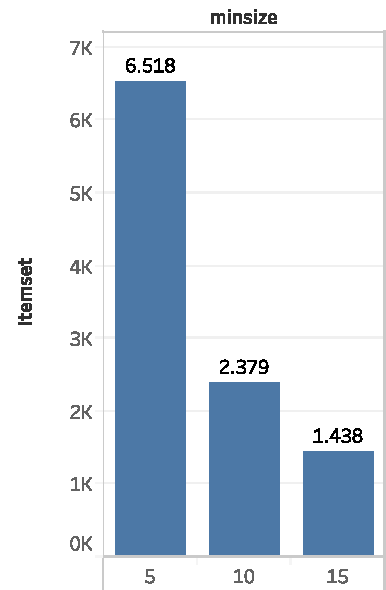
\includegraphics[scale=0.5]{res/fig/sec-4/itemset/ItemsetMinsize.pdf}
   \caption{\(minsize\) tra \(5,10,15\)}
  \label{fig:chap-4:ItemsetMinsize}
\end{subfigure}%
\begin{subfigure}{.5\textwidth}
  \centering
   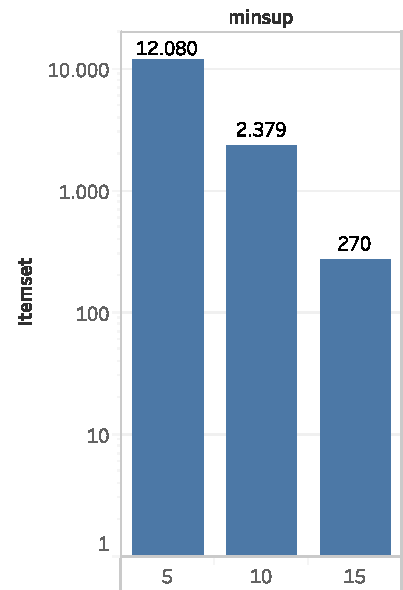
\includegraphics[scale=0.5]{res/fig/sec-4/itemset/ItemsetMinsupp.pdf}
   \caption{\(minsup\)  tra \(5,10,15\)}%
  \label{fig:chap-4:ItemsetMinsupp}
  \end{subfigure}%
  \caption{Numero di itemset alla variazione di \(minsize\) a sinistra e \(minsupp\) a destra}%
  \label{fig:chap-4:ItemsetMinsizeandMinsupp}
\end{figure}

Infine i test condotti su \(\epsilon\) e \(\tau\) mostrano il diverso numero di pattern individuati stringendo o rilassando i vincoli di contiguità.
Per quanto riguarda \(\epsilon\), la \cref{fig:chap-4:ItemsetEpsilon} mostra come il numero di pattern individuati cali al diminuire del valore di soglia.
Questa tendenza rallenta solo nel caso dei valori \(10\) e \(\infty\) dove i risultati quasi coincidono.
I risultati ottenuti su questo parametro sono coerenti con quanto atteso: vincoli più stretti producono meno itemset.
La coincidenza tra il valore \(10\) e \(\infty\) può essere motivata dall'ampiezza del raggio di vicinanza coperto rispetto all'area complessiva del problema.
Un raggio di vicinato pari a \(10\)KM include probabilmente la maggior parte delle celle individuate nello spazio, di conseguenza i suoi risultati tendono a quelli ottenuti rilassando il vincolo.

Per quanto riguarda \(\tau\), è possibile riscontrare come la ricerca di flock, platoon e convoy non produca le differenze attese nei risultati.
Su Geolife le differenze riguardano solo poche tuple tra le tre ricerche.
Questi risultati sono mostrati nella \cref{fig:chap-4:ItemsetTau}.
Questo comportamento è a prima vista inusuale: i vincoli sullo spazio si dimostrano efficaci nella riduzione dello spazio di ricerca mentre quelli sul tempo sono praticamente trascurabili.
Tuttavia occorre considerare la diversità fra la scala spaziale e quella temporale in termini di possibili elementi: quest'ultima infatti ha un range decisamente inferiore rispetto a qualunque scala temporale utilizzata nel corso dei test.
Nel caso di scala giornaliera ad esempio i valori possibili sono \(24\), mentre per quella settimanale sono \(7\).
Come detto nella presentazione di Geolife, i singoli punti hanno frequenze di campionamento molto più elevate della granularità temporale del sistema di riferimento.
Quindi sono poche le traiettorie che hanno una continuità rispetto alle ore del giorno, ancora meno rispetto ai giorni della settimana.

\begin{figure}
  \centering
   \begin{subfigure}{.5\textwidth}
  \centering
    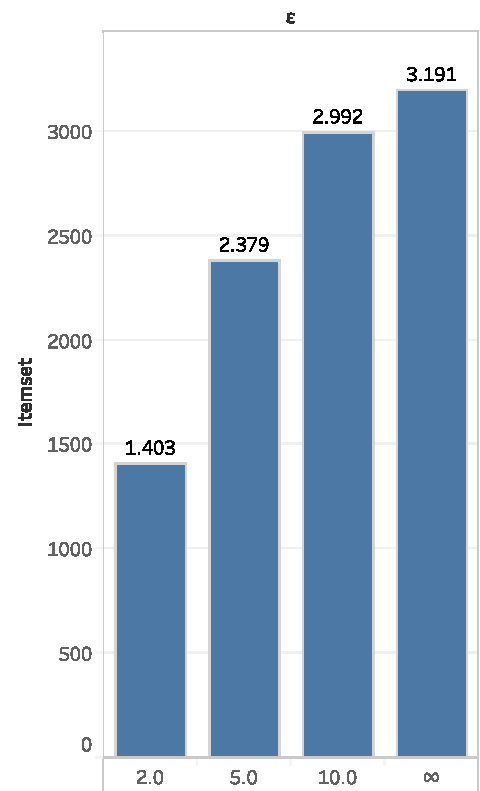
\includegraphics[scale=0.5]{res/fig/sec-4/itemset/ItemsetEpsilon.pdf}
   \caption{\(\epsilon\) tra \(2,5,10,\infty\)}
  \label{fig:chap-4:ItemsetEpsilon}
\end{subfigure}%
\begin{subfigure}{.5\textwidth}
  \centering
   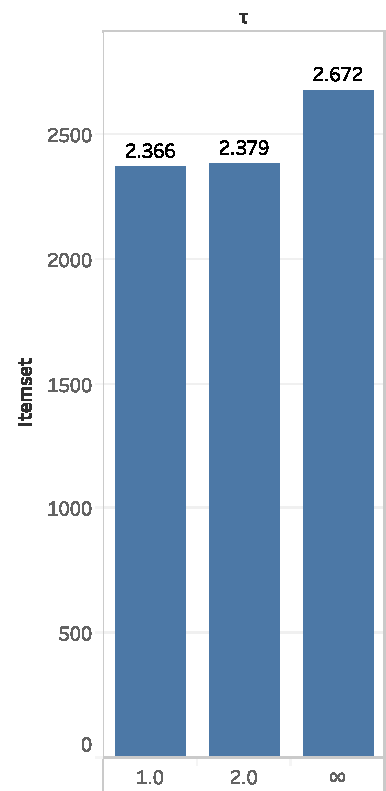
\includegraphics[scale=0.5]{res/fig/sec-4/itemset/ItemesetTau.pdf}
   \caption{\(\tau\) tra \(1,2,\infty\)}%
  \label{fig:chap-4:ItemsetTau}
  \end{subfigure}%
  \caption{Numero di itemset alla variazione di \(\epsilon\) a sinistra e \(\tau\) a destra}%
  \label{fig:chap-4:ItemsetEpsilonAndTau}
\end{figure}




\subsection{Performance}\label{subsec:comp:performance}
In parallelo sono state verificate le performance di CUTE valutando diverse situazioni.
In primo luogo, è stato valutato il tempo di esecuzione rispetto alle configurazioni già presentate nella \cref{subsec:comp:cluster}.
Successivamente sono stati eseguiti test per valutare le tempistiche al variare del numero di risorse fisiche impiegate, ovvero executor e core.
In tutti i test il tempo è sempre registrato in millisecondi.

Nel cronometrare la durata dell'algoritmo, non è considerata la fase di creazione delle tabelle di supporto.
Questo perché le tabelle in questione possono potenzialmente essere create separatamente da CUTE e poi utilizzate dall'algoritmo.
Inoltre a parità di parametri \(s\) e \(t\) una stessa tabella può essere utilizzata da più esecuzioni dell'algoritmo.

Partendo dalle valutazioni basate sull'alterazione dei parametri dell'algoritmo, la \cref{fig:chap-4:TimeSandT} mostrano il tempo di calcolo rispetto alle variazioni dei lati spazio-temporali della cella.
Al crescere di \(s\) (\cref{fig:chap-4:TimeS}), cala il tempo di esecuzione.
Intuitivamente ciò è collegato al numero di celle: celle più grandi e meno numerose corrispondono a meno transazioni da valutare durante la ricerca.
Per \(t\) (\cref{fig:chap-4:TimeT}) la situazione è diversa.
Il trend è inversamente proporzionale al numero di celle: al calare di queste, aumentano i tempi di esecuzione.
Nonostante quindi il numero di celle sia maggiore all'inizio con \(t=24h\), la minor lunghezza delle transazioni porta a generare un minor numero di gruppi da esplorare (come evidenziato anche negli itemset individuati) e causa quindi una diminuzione nei tempi di esecuzione.

\begin{figure}
  \centering
  \begin{subfigure}{.5\textwidth}
  \centering
   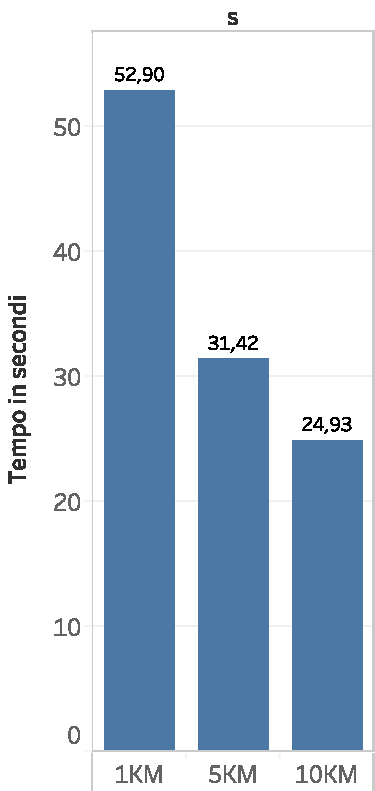
\includegraphics[scale=0.5]{res/fig/sec-4/performance/TimeS.pdf}
   \caption{\(s\) tra \(1,5,10\) KM}
  \label{fig:chap-4:TimeS}
\end{subfigure}%
\begin{subfigure}{.5\textwidth}
  \centering
   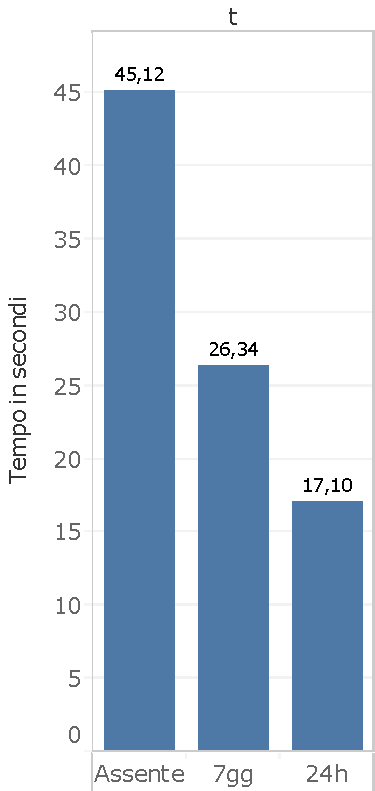
\includegraphics[scale=0.5]{res/fig/sec-4/performance/TimeT.pdf}
   \caption{\(t\) tra 24h, 7gg e assenza di tempo}
  \label{fig:chap-4:TimeT}
\end{subfigure}%
  \caption{Tempo di computazione alla variazione di \(s\) a sinistra, \(t\) a destra}%
  \label{fig:chap-4:TimeSandT}
\end{figure}

Variando \(minsize\) (\cref{fig:chap-4:TimeMinsize}) è possibile vedere un trend di diminuzione dei tempi di esecuzione al crescere del parametro.
Questo è coerente con quanto atteso: la ricerca di gruppi più numerosi comporta il pruning dei piccoli gruppi e risparmia tempo sul tempo di esecuzione globale.
Considerando invece \(minsup\) (\cref{fig:chap-4:TimeMinsupp}), vale lo stesso discorso.
Le ragioni sono analoghe a quanto detto per \(minsize\).


\begin{figure}
  \centering
   \begin{subfigure}{.5\textwidth}
  \centering
    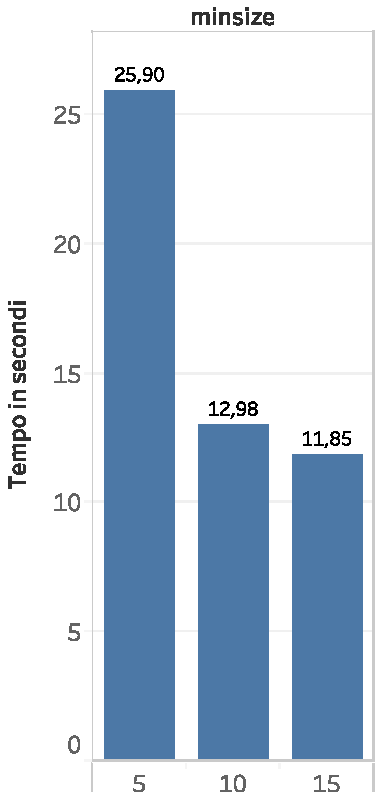
\includegraphics[scale=0.5]{res/fig/sec-4/performance/TimeMinsize.pdf}
   \caption{\(minsize\) tra \(5,10,15\)}
  \label{fig:chap-4:TimeMinsize}
\end{subfigure}%
\begin{subfigure}{.5\textwidth}
  \centering
   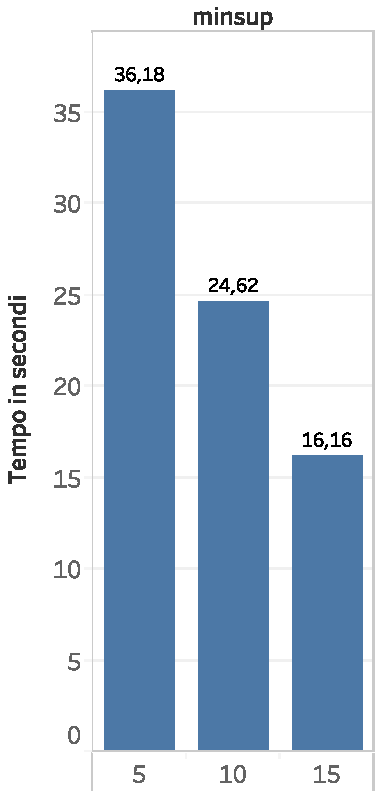
\includegraphics[scale=0.5]{res/fig/sec-4/performance/TimeMisupp.pdf}
   \caption{\(minsup\) tra \(5,10,15\)}%
  \label{fig:chap-4:TimeMinsupp}
  \end{subfigure}%
  \caption{Tempo di computazione alla variazione di \(minsize\) a sinistra e \(minsupp\) a destra}%
  \label{fig:chap-4:TimeMinsizeandMinsupp}
\end{figure}

Trattando poi dei parametri di continuità che riducono lo spazio di ricerca, \(\epsilon\) (\cref{fig:chap-4:TimeEpsilon}) presenta per entrambi i dataset una certa regolarità: al crescere del suo valore, aumenta il tempo di computazione.
Questa regolarità dipende dalla riduzione dello spazio di ricerca effettuato dai vincoli.
Valori più rigidi comportano una maggior riduzione dello spazio di ricerca, che si traduce in un pruning più forte

Su \(\tau\) (\cref{fig:chap-4:TimeTau}) la situazione è più eterogenea: non è possibile individuare un trend definito.
Ancora una volta le cause sono da ricercare nel debole pruning di \(\tau\), la presenza di questo vincolo infatti può in ceri casi rallentare l'esecuzione, in quanto giunge a risultati assimilabili a quelli ottenuti rilassando il vincolo.
Questa ricerca avviene in maniera più lenta, per via delle operazioni aggiuntive sul controllo della continuità.

\begin{figure}
  \centering
   \begin{subfigure}{.5\textwidth}
  \centering
    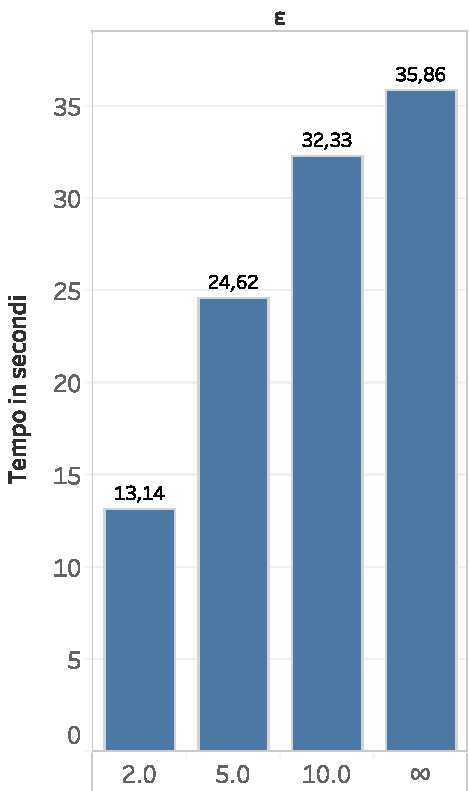
\includegraphics[scale=0.5]{res/fig/sec-4/performance/TimeEpsilon.pdf}
   \caption{\(\epsilon\) tra \(2,5,10,\infty\)}
  \label{fig:chap-4:TimeEpsilon}
\end{subfigure}%
\begin{subfigure}{.5\textwidth}
  \centering
   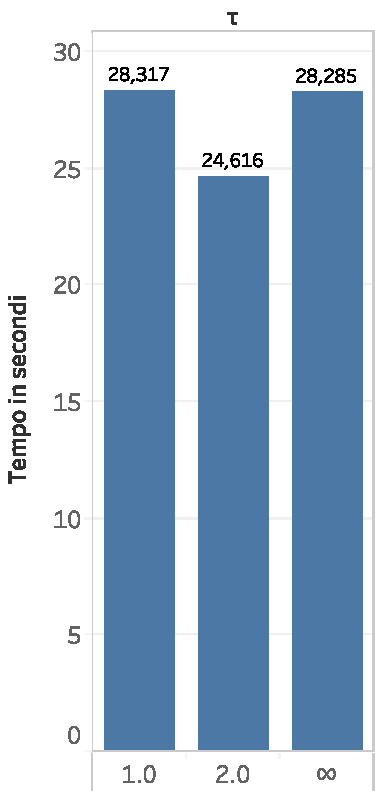
\includegraphics[scale=0.5]{res/fig/sec-4/performance/TimeTau.pdf}
   \caption{\(\tau\) tra \(1,2,\infty\)}%
  \label{fig:chap-4:TimeTau}
  \end{subfigure}%
  \caption{Tempo di computazione alla variazione di \(\epsilon\) a sinistra e \(\tau\) a destra}%
  \label{fig:chap-4:TimeEpsilonAndTau}
\end{figure}

Passando ai test di scalabilità, questi sono stati condotti su un sottoinsieme dei parametri utilizzati nella sezione precedente.
Ciascuna configurazione di parametri è stata testata variando rispettivamente il numero di executor  e quello di core, mantenendo come altri parametri i valori di default specificati nella \cref{tab:parameters-variation}.
La \cref{tab:cores-executors-variation} contiene i valori possibili per core e executor.

\begin{table}[H]
    \centering
   \begin{tabular}{||c c||}
 \hline
     Parametro & Valori \\ [0.4ex] 
 \hline\hline
   core & 2,\textbf{3},4 \\
 \hline
  executor & 5,\textbf{7},9 \\
 \hline
\end{tabular}
    \caption{Valori per core e executor (default in grassetto)}
    \label{tab:cores-executors-variation}
\end{table}


Le \cref{fig:chap-4:ScalabilityCORES,fig:chap-4:ScalabilityEXECUTORS}
mostrano i tempi di esecuzione alla variazione di questi parametri.

\begin{figure}
  \centering
   \begin{subfigure}{.5\textwidth}
  \centering
      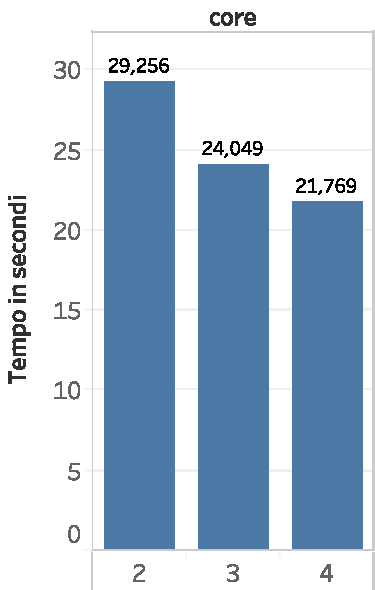
\includegraphics[scale=0.5]{res/fig/sec-4/scalability/ScalabilityDataCORES.pdf}
  \caption{core tra \(2,3,4\)}%
  \label{fig:chap-4:ScalabilityCORES}
\end{subfigure}%
\begin{subfigure}{.5\textwidth}
  \centering
   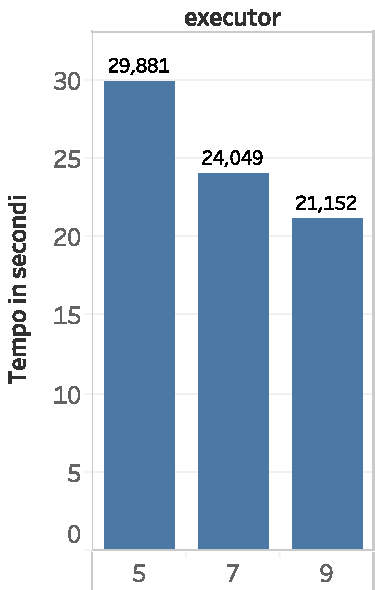
\includegraphics[scale=0.5]{res/fig/sec-4/scalability/ScalabilityDataEXECUTORS.pdf}
  \caption{executor tra \(5,7,9\)}%
  \label{fig:chap-4:ScalabilityEXECUTORS}
  \end{subfigure}%
  \caption{Tempo di computazione alla variazione di core a sinistra e executor a destra}%
  \label{fig:chap-4:ScalabilityCORESandEXECUTORS}
\end{figure}

Com'è possibile notare, la tendenza generale espressa dai grafici è una diminuzione dei tempi di esecuzione all'aumentare dell'impiego di risorse.

Infine per quanto riguarda l'ambito delle performance, sono stati eseguiti alcuni test di scalabilità rispetto al numero di traiettorie.
In particolare per questi è stato utilizzato Oldenburg, in quanto avente un numero di traiettorie molto superiore a Geolife.
La \cref{tab:variation-oldenburg} contiene i parametri di CUTE utilizzati durante queste esecuzioni.

\begin{table}[H]
    \centering
   \begin{tabular}{||c c||}
 \hline
     Parametro & Valore \\ [0.4ex] 
 \hline\hline
 traiettorie & \(50\)K,\(500\)K,\(1.000\)K \\
 \hline
 \(s\) & 1000 \\
 \hline
 \(t\) & 10 \\
 \hline
 \(minsize\) & 100 \\
 \hline
  \(minsupp\) & 10 \\
 \hline
  \(\epsilon\) & \(2\) \\
 \hline
 \(\tau\) & \(1\) \\
 \hline
   core & 3 \\
 \hline
  executor & 9 \\
 \hline
\end{tabular}
    \caption{Valori dei parametri di CUTE utilizzati durante i test sul numero di traiettorie su Oldenburg}
    \label{tab:variation-oldenburg}
\end{table}

I risultati indicano come a parità di risorse, CUTE riesca a gestire in tempi ragionevoli anche un numero di transazioni molto elevato (\cref{fig:chap-4:ScalabilityOldenburg}).
Nel caso peggiore infatti sono necessarie appena 10 minuti per eseguire la ricerca su un milione di traiettorie.
Questo dipende da diversi fattori.
In primo luogo il numero di celle, e di conseguenza quello di transazioni, rimane invariato durante le varie esecuzioni.
Ciò che cambia è quindi la lunghezza media di ogni transazione, che aumenta all'aumentare del numero di traiettorie.
Insiemi di transazioni di diversi ordini di grandezza vengono processati in diversi ordini temporali di grandezza.
Oltre a ciò, questi risultati possono essere collegati a valori molto stringenti per i parametri collegati al pruning, dimostrando così la loro efficacia nel ridurre lo spazio di ricerca.



\begin{figure}
  \centering
  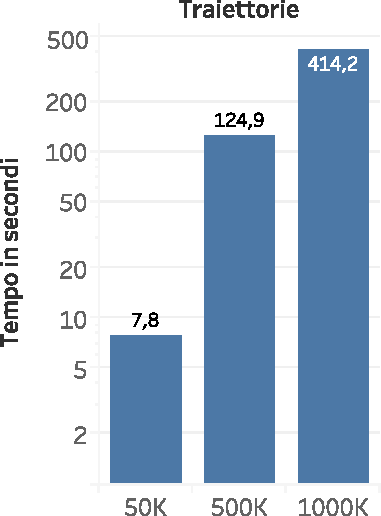
\includegraphics[scale=.5]{res/fig/sec-4/performance/ScalabilityOnOldenburg.pdf}
  \caption{Tempi di esecuzione in secondi variando il numero di traiettorie tra \(50\)K,\(500\)K,\(1000\)K}%
  \label{fig:chap-4:ScalabilityOldenburg}
\end{figure}



\subsection{Considerazioni}\label{subsec:comp:consideration-and-limits}
Alla luce di quanto mostrato riguardo a itemset individuati e performance, si possono trarre le seguenti considerazioni.

In primo luogo i risultati ottenuti confermano l'importanza della suddivisione in quanti sulla base del sistema di riferimento. 
Questo è un aspetto delicato. 
La grana del sistema di riferimento è direttamente collegata con il tipo di pattern che si vuole ricercare.
Differenti ricerche infatti possono portare a differenti suddivisioni dello spazio di ricerca.
Ad esempio una ricerca che consideri la rete stradale di una città avrà sempre molti più quanti di una che considera i quartieri o municipalità di una città.
Occorre quindi valutare il comportamento rispetto alla variazione di transazioni in input e al sistema di riferimento.
Per simulare questo scenario, sono state utilizzate più griglie che hanno permesso di costruire di volta in volta un numero di transazioni arbitrario.

Dai test svolti è emerso che il comportamento dell'algoritmo al variare del numero di celle può essere riassunto come segue:
Per ogni dataset, esiste un sistema di riferimento ideale avente una certa granularità.
Nell'utilizzo di griglie a grana più grossa, a parità di dimensione e supporto minimo, calano le transazioni di esplorare.
Di conseguenza calano gli itemset validi (per via del supporto) e i tempi di esecuzione.
Usando griglie a grana troppo fine, il numero di transazioni aumenta, ma diminuisce la lunghezza di ogni transazione.
In questo caso è la frammentazione a ridurre il numero di elementi in ogni transazione, diminuendo quindi il supporto e la dimensione media degli itemset individuati.
Questo comporta un maggiore pruning e di conseguenza una riduzione nei tempi di calcolo e negli itemset trovati.
In entrambi questi due casi, il sistema di riferimento risulta scarsamente compatibile con le caratteristiche spazio-temporali del dataset.

Per quanto riguarda i parametri di supporto \(minsup\) e dimensione \(minsize\), il comportamento dell'algoritmo è in linea con quanto atteso in ogni situazione.
L'aumentare dei due parametri comporta una riduzione degli itemset validi.
Il pruning di questi itemset diminuisce il volume della ricerca e di conseguenza il costo computazionale totale. 

Altro punto focale emerso dai test è la debolezza nel vincolo di continuità temporale negli itemset individuati: rispetto a quello spaziale infatti il pruning effettuato è molto più debole.
Come già affermato precedentemente, questo dipende dalla finezza della scala impiegata.
Per quanto riguarda la componente spaziale, è improbabile che traiettorie vicine si muovano su celle lontane della mappa.
Per il tempo invece, come affermato nella \cref{subsec:comp:cluster}, le scale delle ore/giorni risultano poco compatibili con l'alto tempo di campionamento delle traiettorie.
Sempre collegato ai vincoli di continuità e alla riduzione dello spazio di ricerca, non sempre accade che una riduzione dello spazio di ricerca comporti un calo nei tempi di esecuzione.
Come affermato nella \cref{subsec:cute:ctm}, il rilassamento dei vincoli sulla continuità nello spazio tempo rende superflue alcune operazione e rende più snella la computazione.
Se quindi il pruning effettuato da questi vincoli è debole, lo spazio di ricerca non sarà ridotto e sarà esplorato più lentamente per via dei vincoli.
Oltre a questo, dal punto di vista implementativo la ricerca di swarm produce meno job da eseguire.
Ogni job spark infatti aggiunge una costo computazionale alla ricerca, in quanto richiede un certo overhead in termini di tempo e risorse per essere creato.

CUTE, come mostrato dai test di scalabilità, ottiene tempi ragionevoli con diverse configurazioni di risorse.
Ciò è possibile grazie al numero contenuto di celle individuate, che risulta sempre molto minore del numero di traiettorie.
Qualora si adottasse una scala temporale assoluta o si riducesse di molto l'area spaziale coperta dalla singola cella, le performance di CUTE calerebbero notevolmente.
La ragione dietro questo calo sarebbe attribuibile all'esplosione del numero di celle.
Con un numero alto di celle, non solo la creazione delle tabelle di supporto aumenta esponenzialmente, ma vengono meno i principi del mining su dataset colossali, in quanto il numero di transazioni (celle) supera quello di item (traiettorie).

\section{CUTE vs SPARE}\label{sec:CUTEvsSPARE}
Terminata l'analisi di CUTE in termini di itemset e tempo di computazione, si passa al confronto tra CUTE e SPARE.
Gli algoritmi approcciano uno stesso problema, la ricerca di pattern di co-movimento, con due tecniche differenti tra di loro.
Questo comporta che durante un confronto, non abbia senso parlare di tempistiche: CUTE e SPARE sono intrinsecamente diversi e la velocità non può essere un buon metro di confronto.
Se il tempo di esecuzione non può essere utilizzato, allora l'intero confronto sarà impostato sulla base dei pattern ottenuti tra i due algoritmi.

\subsection{Confronto tra CUTE e SPARE}\label{subsec:comp:CUTEvsSPARE}
CUTE e SPARE entrambi eseguono una ricerca di pattern di co-movimento.
In tutti e due sono presenti i concetti di lunghezza minima del percorso (\(k, \alpha\)), dimensione minima di un gruppo (\(m, \gamma\)) e massimo gap temporale tra i punti del percorso (\(g, \tau\)).

Parlando poi delle idee di funzionamento dei due algoritmi, in entrambi si utilizzano i concetti di itemset,pruning e monotonicità. 
In CUTE ciò viene realizzato dividendo lo spazio di ricerca in celle, assegnando a ogni cella l'insieme delle traiettorie che transitano nei suoi confini spazio-temporali e eseguendo poi una variante distribuita dell'algoritmo di Carpenter per ricercare cluster di traiettorie.
SPARE invece utilizza un approccio basato su itemset solo nella seconda fase, quella relativa al tempo e formula una propria definizione di monotonicità, diversa dalla frequenza, basata su due parametri \(l\) e \(g\).
Nella prima fase utilizza un clustering spaziale per definire ad ogni istante quali punti sono vicini e quali no.

SPARE prende come ipotesi che per ogni istante della scala temporale, ogni traiettoria abbia al massimo una posizione: questo diventa limitante quando si vuole considerare traiettorie generate da diverse scale di campionamento, poiché l'algoritmo riduce tutte le traiettorie a una scala comune.
Questo processo di semplificazione comporta una perdita di informazioni.

Anche su CUTE è necessario compiere un'operazione di assimilazione a una stessa scala temporale, tuttavia CUTE pone l'enfasi della sua divisione nella creazione di celle con un certo volume nello spazio-tempo.
Dal punto di vista temporale, ogni cella non esprime un istante, ma una durata.
Una traiettoria passa da una cella se transita nei suoi confini anche solo per un istante.
Questo implica che una traiettoria possa muoversi su un range di celle aventi stesso istante temporale.
In questo modo CUTE minimizza la perdita di informazione legata all'adozione di una scala temporale univoca su diverse traiettorie.

Dal punto di vista della vicinanza nello spazio, SPARE è più flessibile sulle forme dei cluster, potendo utilizzare vari algoritmi differenti per la creazione di questi.
Al contrario CUTE ha confini spaziali più rigidi, determinati da una divisione regolare dello spazio.
SPARE però considera la vicinanza solo in termini relativi, trascurando i movimenti eseguiti dal gruppo tra due istanti temporali.
CUTE invece permette di esprimere vincoli sulla contiguità spaziale (\(\epsilon\)) tra le varie celle percorse da un gruppo.

Parlando poi della dimensione temporale, CUTE presenta una gestione omogenea rispetto alla dimensione spaziale, processando quindi spazio e tempo assieme, tuttavia l'algoritmo mostra i suoi limiti in corrispondenza di bucket temporali nell'ordine dei secondi o pochi minuti, a causa dell'aumento del numero di celle. 
SPARE invece ha buone performance anche con bucket temporali nell'ordine dei secondi, inoltre permette una maggiore espressività nei vincoli temporali grazie al vincolo \(l\).
Dall'altro lato però CUTE è in grado di gestire scale temporale cicliche come i giorni della settimana o le ore del giorno, mentre SPARE è limitato a una scala temporale monotona.

CUTE consente inoltre di processare altre dimensioni senza nessuna ulteriore espansione, mentre SPARE è pensato esclusivamente solo per processare dati spazio-temporali.

Trattando infine i risultati, SPARE genera cluster basati su itemset frequenti massimali, CUTE invece su frequenti chiusi. 
CUTE quindi, a parità di configurazione, genererà sempre un numero maggiore di risultati rispetto a SPARE.

\subsection{Risultati a parità di configurazione}\label{subsec:comp:result-comparison}
Come detto nella sezione precedente, CUTE individua itemset chiusi, SPARE massimali.
Per quanto molti passi nei due approcci divergano, è possibile in determinate condizioni ottenere gli stessi risultati tra i due algoritmi.
Ciò però avviene solo in casistiche particolari, nella maggior parte delle situazioni succede che i risultai divergano per alcune caratteristiche intrinseche dei due algoritmi:

\begin{itemize}
    \item \textit{Itemset chiusi \(\supseteq\) Itemset massimali}. È fisiologico, salvo rare eccezioni, che il numero di itemset chiusi in un dataset sia anche di ordini di grandezza più grande di quello dei massimali.
    \item \textit{Le metriche spaziali divergono}.
   L'impiego di due metriche spaziali differenti porta a risultati che in assoluto possono divergere per alcune tuple.
\end{itemize}

Per quanto i due algoritmi possano avere elementi in comune, queste particolarità devono essere tenute in conto durante il confronto dei risultati.
Confrontare il numero di itemset identici produrrebbe quindi scarsi risultati.
Serve perciò definire una metrica di confronto che tenga conto di queste due caratteristiche: non deve penalizzare eccessivamente la differenza nel numero dei risultati e deve misurare la similarità tra gli itemset tenendo conto che questi possono divergere per l'assenza o presenza di qualche elemento.

Alla luce di questo, è stata formulata la seguente misura di similarità \(S\).
Per confrontare i due insiemi di itemset si utilizza una variazione dello Stable Marriage Problem~\cite{mcvitie1971stable}.
Dati due set di stesse dimensioni, questa tecnica permette di assegnare ogni elemento di un set a uno dell'altro sulla base di un criterio di similarità custom.
Questo permette di ottenere una soluzione sub-ottima al problema dell'assegnamento, assicurandosi che non esistano due elementi appartenenti a insiemi diversi che abbiano una similarità maggiore tra di loro rispetto che coi rispettivi partner (\cref{definition:stable-marriage-problem}).

\begin{definition}[Stable Marriage Problem]\label{definition:stable-marriage-problem}

 Dati due insiemi di oggetti \(N\) e \(M\), si definisce problema del matrimonio stabile il problema che ricerca l'insieme delle coppie \((n_i \in N, m_j \in M)\) tali che definita una metrica di similarità \(s\) non esistano in contemporanea due coppie \((n_p, m_p),(n_q,m_q)\) tali che  \(n_p,n_q \in N,m_p,m_q \in M\) per cui vale che: 
  \begin{center}
  \(
    \begin{cases}
     s(n_p,m_j) > s(n_i, m_j) \land s(n_p,m_j) > s(n_p,m_p) \\
     s(n_i, m_q) > s(n_i, m_j) \land s(n_i, m_q) > s(n_q, m_q)
    \end{cases}
    \)
  \end{center}
\end{definition}

Definita la modalità di assegnamento, si rende necessario individuare una metrica di confronto tra i singoli itemset.
Questa è definita via coefficiente di Jaccard.
Questo calcola la similarità tra due set come il numero di elementi condivisi tra i due diviso l'unione di tutti gli elementi presenti in entrambi (\cref{definition:jaccard}).

\begin{definition}[Coefficiente di Jaccard]\label{definition:jaccard}

 Dati due set di item \(N\) e \(M\), si definisce il coefficiente di Jaccard tra i due insiemi come: 
    \begin{center}
        \(Jaccard(N,M) = \frac{|N \cap M|}{|N \cup M|}\) 
    \end{center}
\end{definition}

Una volta definita questa metrica, la similarità totale \(S\) tra i risultati di CUTE e SPARE viene calcolata nel seguente modo:
in primo luogo viene eseguito l'assegnamento di ogni cluster individuato su un algoritmo a quello di un altro sulla base del valore di Jaccard tra i due.
Questa operazione segue le regole del problema del matrimonio stabile, di conseguenza produce una soluzione sub-ottima.
A questo punto viene calcolata la somma totale dei valori di similarità tra ogni coppia e questo risultato viene poi diviso per il numero delle coppie totali.
Il risultato di questa operazione determina la similarità tra due insiemi.

\begin{definition}[Similarità tra due set di cluster]\label{definition:cluster-similarity}

Dato un set di cluster di CUTE \(C\), uno di SPARE \(M\) e insieme di coppie \(CM = \{(c_1, m_1), \ldots, (c_n, m_n)\}\), generato mediante risoluzione del problema del matrimonio stabile utilizzando \(Jaccard\) come metrica di similarità, tali che \( c_ i \in C \land m_i \in M\) si definisce la similarità \(S\) con la seguente formula:

  \begin{equation}
     S(C, M) = \frac{\sum_{k=1}^{n}{Jaccard(c_k, m_k)}}{n} 
    \end{equation}

\end{definition}

Occorre però un'ulteriore precisazione.
Come detto sopra il problema del matrimonio stabile funziona solo se entrambi gli insiemi hanno lo stesso numero di elementi.
CUTE e SPARE invece divergono per numero di itemset: in particolare CUTE individuerà in media molti più risultati di SPARE.
Per risolvere questo problema, sono state definite due variazioni della metrica: in una gli elementi in più sono scartati \((S_{minus})\) mentre nell'altra \((S_{plus})\) contribuiscono alla misura con un valore di similarità pari a \(0\).
Tra queste due metriche ci è sembrato più rilevante cercare di massimizzare \((S_{minus})\), in quanto misura che penalizza in maniera minore la differenza di cardinalità tra massimali e chiusi.

Definita la procedura di confronto, è stato scelto come dataset utilizzato Oldenburg, campionato ogni \(5\) istanti temporali.
Questa configurazione garantisce che il numero di celle create da CUTE aumenta in maniera controllata, allo stesso tempo il dataset rimane abbastanza compatto per ottenere risultati significativi rispetto a SPARE.

I primi test sono stati condotti sul dataset nella sua interezza, a parità di risorse fornite.
CUTE sin da subito è stato in grado di gestire la complessità del problema nel suo insieme, mentre SPARE no.
In numerose occasioni, le risorse fornite all'applicazione non sono state sufficienti per permettere all'algoritmo di terminare con successo.

Alla luce di questi fallimenti, è stato ridotto il numero di traiettorie impiegate.
Sono stati così condotti esperimenti su \(1000, 2000\) e infine \(3000\) traiettorie.
Anche in queste condizioni, SPARE ha avuto difficoltà nell'eseguire la ricerca con determinate configurazioni.
Inoltre la differenza tra i risultati dei due algoritmi risultava decisamente grande: in alcune situazioni SPARE individuava \(1\text{-}2\) elementi, mentre CUTE sui \(1000\text{-}2000\).

Sono state impiegate allora tecniche e accorgimenti per riuscire a ottenere risultati significativi.
Il primo passo è stato individuare una configurazione di \(\epsilon, minPts\) che permettesse a SPARE di individuare un numero consistente di itemset (\(> 50\)) su più configurazioni.
Successivamente è stato lanciato diverse volte CUTE, variando il lato spaziale delle celle su valori ragionevoli e direttamente collegati a \(\epsilon\).
Di seguito (\cref{fig:chap-4:CompM,fig:chap-4:CompK,fig:chap-4:CompG,fig:chap-4:CompS}) è illustrato il confronto tra SPARE e CUTE.
La \cref{tab:comparison-variation} riassume le configurazioni di parametri in gioco.

\begin{table}[H]
    \centering
   \begin{tabular}{||c c c||}
 \hline
     Parametro & Algoritmo & Valori \\ [0.4ex] 
 \hline\hline
   \(s\) & CUTE & \(1.5,\textbf{1.75},2\) KM \\
 \hline
  \(\epsilon\) & SPARE & \(\textbf{2}\) KM \\
 \hline
 \(minPoints\) & SPARE & \(\textbf{5}\) \\
 \hline
 \(m\) & SPARE e CUTE & \(3,\textbf{4},5\) \\
 \hline
 \(k\) & SPARE e CUTE & \(4,\textbf{5},10\) \\
 \hline
 \(g\) & SPARE e CUTE & \(2,\textbf{5},1000\) \\
 \hline
\end{tabular}
    \caption{Valori dei parametri in gioco durante il confronto (default in grassetto)}
    \label{tab:comparison-variation}
\end{table}

\begin{figure}
  \centering
   \begin{subfigure}{.5\textwidth}
  \centering
      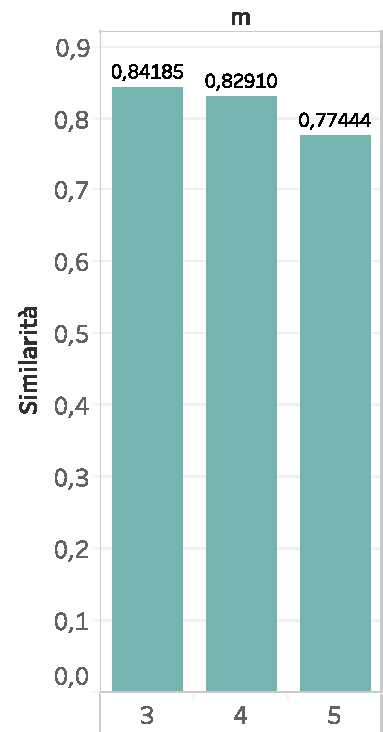
\includegraphics[scale=0.6]{res/fig/sec-4/scalability/ComparisonMSimilarity.pdf}
  \caption{Similarità \(S_{minus}\)}%
\end{subfigure}%
\begin{subfigure}{.5\textwidth}
  \centering
   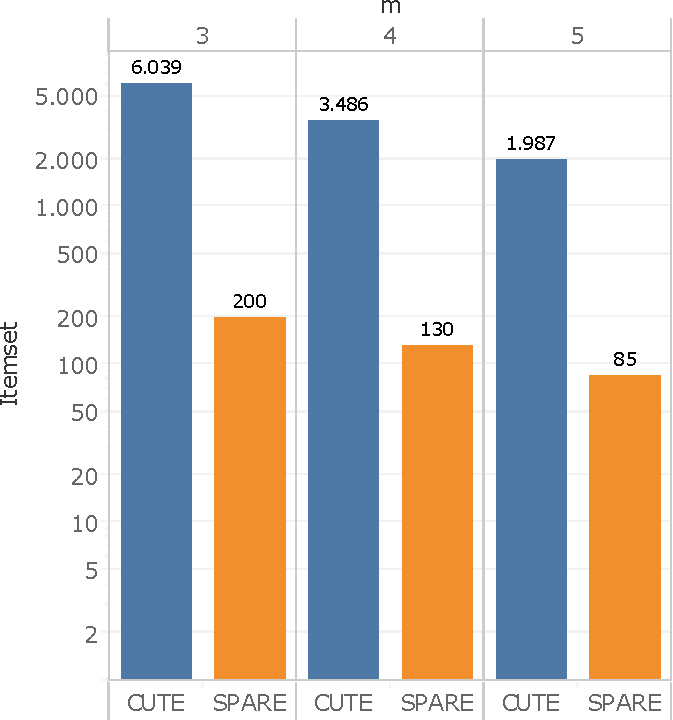
\includegraphics[scale=0.6]{res/fig/sec-4/scalability/ComparisonMCUTESPARE.pdf}
  \caption{Itemset individuati su CUTE e SPARE}%
  \end{subfigure}%
  \caption{Similarità a sinistra, itemset a destra al variare della dimensione minima dei gruppi \(m\)}%
  \label{fig:chap-4:CompM}
\end{figure}

\begin{figure}
  \centering
   \begin{subfigure}{.5\textwidth}
  \centering
      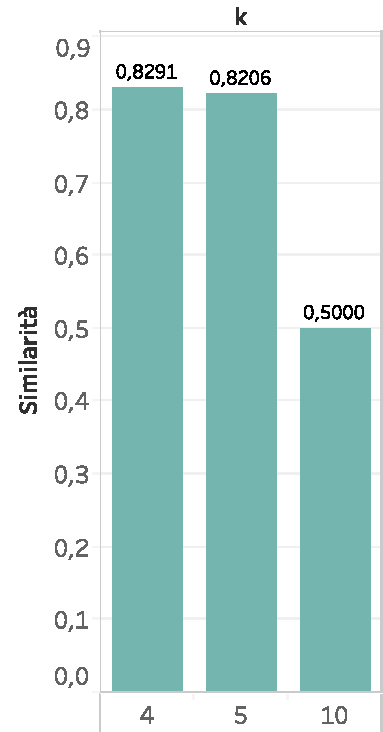
\includegraphics[scale=0.6]{res/fig/sec-4/scalability/ComparisonKSimilarity.pdf}
  \caption{Similarità \(S_{minus}\)}%
\end{subfigure}%
\begin{subfigure}{.5\textwidth}
  \centering
   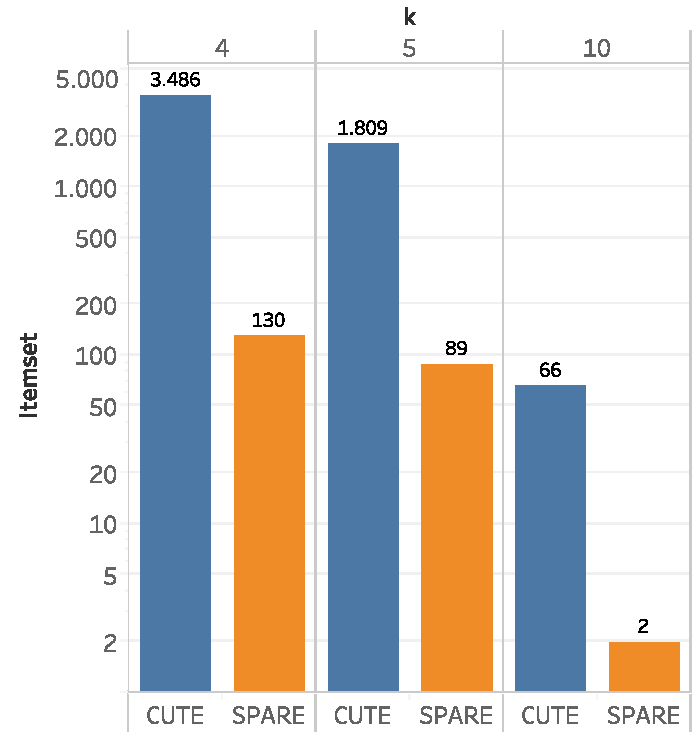
\includegraphics[scale=0.6]{res/fig/sec-4/scalability/ComparisonKCUTESPARE.pdf}
  \caption{Itemset individuati su CUTE e SPARE}%
  \end{subfigure}%
  \caption{Similarità a sinistra, itemset a destra al variare del supporto minimo \(k\)}%
  \label{fig:chap-4:CompK}
\end{figure}


Al variare di \(m\) (\cref{fig:chap-4:CompM}), è possibile vedere come all'aumentare delle dimensioni dei gruppi, la similarità totale tenda a calare.
Discorso analogo vale per \(k\): al suo aumentare la similarità totale cala.
Questo può essere giustificato sulla base delle divergenze nel determinare la vicinanza spaziale tra i due algoritmi.
Impostando infatti vincoli più rigidi, verranno riconosciuti itemset con maggiori dimensioni e supporto.
All'aumento di queste due misure corrisponde un incremento della possibilità che la composizione dei gruppi individuati tra i due algoritmi cambi.

Trattando invece di \(g\) \cref{fig:chap-4:CompG}, al rilassamento della continuità aumenta la similarità.
Anche questo è collegato con quanto detto sopra: pattern swarm contenenti gli stessi oggetti possono essere individuati in situazioni differenti.
È più raro che ciò possa accadere invece con pattern continui nel tempo, come ad esempio flock.

\begin{figure}
  \centering
   \begin{subfigure}{.5\textwidth}
  \centering
      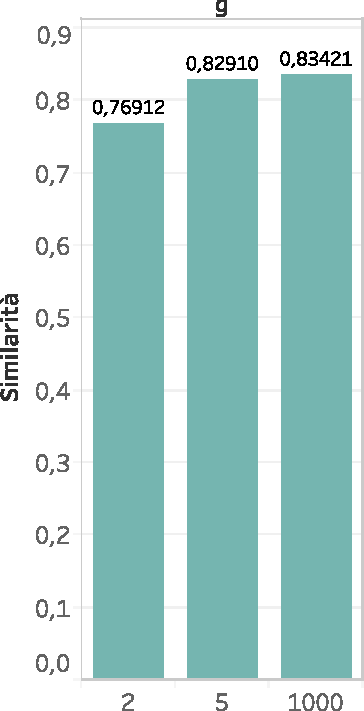
\includegraphics[scale=0.6]{res/fig/sec-4/scalability/ComparisonGSimilarity.pdf}
  \caption{Similarità \(S_{minus}\)}%
\end{subfigure}%
\begin{subfigure}{.5\textwidth}
  \centering
   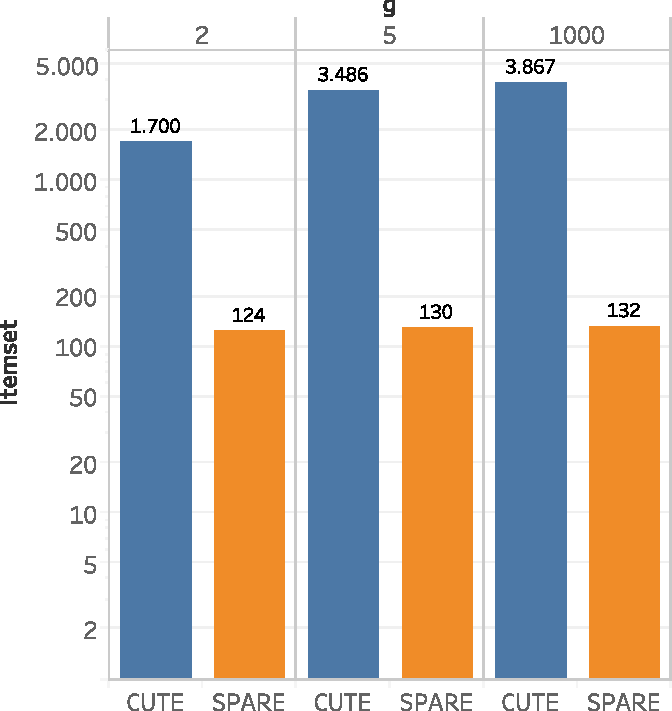
\includegraphics[scale=0.6]{res/fig/sec-4/scalability/ComparisonGCUTESPARE.pdf}
  \caption{Itemset individuati su CUTE e SPARE}%
  \end{subfigure}%
  \caption{Similarità a sinistra, itemset a destra al variare della continuità sul tempo \(g\)}%
  \label{fig:chap-4:CompG}
\end{figure}

Infine al variare di \(s\) si può vedere come il valore di similarità migliore si ottenga con il valore medio di \(s\).
La spiegazione di ciò può essere ricondotta alla distribuzione dei dati nello spazio.
Purtroppo è difficile determinare con precisione il valore ottimale di \(s\), se non determinandolo sperimentalmente.
Nonostante questo, \(1.75\) risulta un buon valore: quasi il \(50\%\) degli itemset di SPARE sono coperti da CUTE e la similarità complessiva è dell'\(80\%\). 

\begin{figure}
  \centering
   \begin{subfigure}{.5\textwidth}
  \centering
      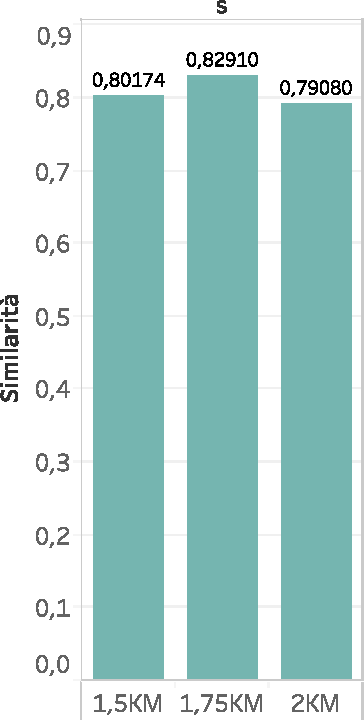
\includegraphics[scale=0.6]{res/fig/sec-4/scalability/ComparisonSSimilarity.pdf}
  \caption{Similarità \(S_{minus}\)}%
\end{subfigure}%
\begin{subfigure}{.5\textwidth}
  \centering
   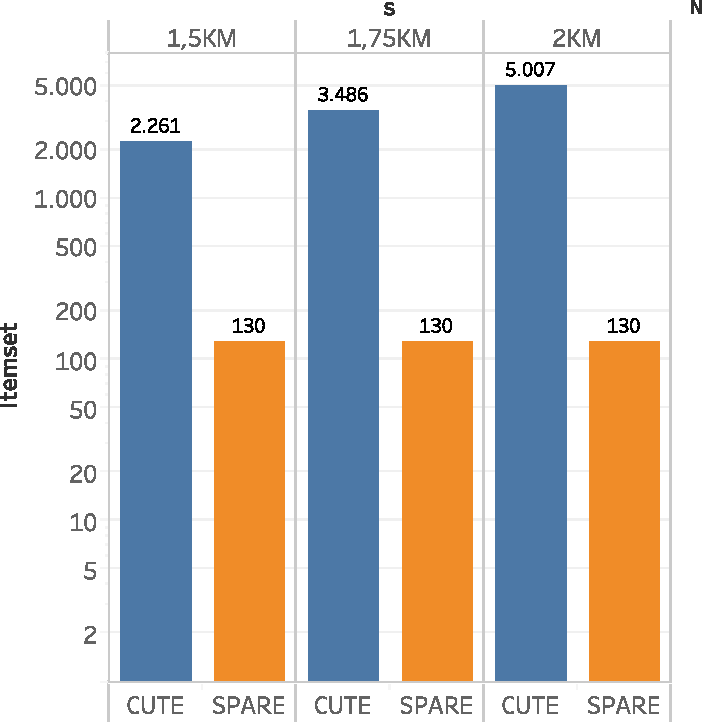
\includegraphics[scale=0.6]{res/fig/sec-4/scalability/ComparisonSCUTESPARE.pdf}
  \caption{Itemset individuati su CUTE e SPARE}%
  \end{subfigure}%
  \caption{Similarità a sinistra, itemset a destra al variare dell'area spaziale coperta dalle celle \(s\)}%
  \label{fig:chap-4:CompS}
\end{figure}


\subsection{Interpretazione dei risultati}\label{subsec:comp:result-evaluation}
Anche utilizzando definizioni di similarità personalizzate sul problema, i risultati fra i due cluster sono comunque molto diversi fra di loro.

Sicuramente entrambi gli algoritmi formalizzano la ricerca di pattern di co-movimento con alcuni elementi in comune, tuttavia l'approccio alla ricerca e la natura stessa degli itemset individuati porta a escludere una casistica reale in cui gli algoritmi individuano esattamente gli stessi cluster.
È però possibile tentare di massimizzare l'intersezione tra i risultati di questi due algoritmi, sempre tenendo presente che le cardinalità di CUTE sono di molto superiori a quelle di SPARE.

In teoria a parità di risultati sul clustering spaziale dovrebbe garantire quanto meno la totale sovrapposizione totale dei risultati di SPARE su quelli di CUTE.
Questo perché il tempo viene processato nello stesso modo dai due algoritmi, mentre invece lo spazio no.
Tuttavia trovare questo punto di intersezione è praticamente impossibile, SPARE valuta i cluster ad ogni istante temporale, definendo potenzialmente una configurazione spaziale diversa ad ogni istante.
La divisione effettuata da CUTE invece è fissa in tutti gli istanti temporali.

Sia CUTE che SPARE dispongono poi di vincoli che l'altro non non è in grado di coprire.
Questi devono essere necessariamente rilassati durante il confronto, per non far divergere ulteriormente i risultati.
Ciò però implica che il potenziale espressivo di questi parametri sia perso nella ricerca.

In definitiva CUTE e SPARE pongono due approcci che possono convergere parzialmente nella ricerca di pattern di co-movimento.
Allo stesso tempo tuttavia portano un contributo unico alla ricerca che viene minimizzato quando si vuole far convergere i risultati.





%---------------- TIME TEST











%------------- SCALABILITY TEST






%------- COMPARISON TEST





  \chapter{Conclusioni e sviluppi futuri}\label{chapter:chapter5}
  Il contributo fornito da questa tesi si spinge nell'analisi approfondita del clustering di traiettorie e del frequent itemset mining.
Durante questa analisi è stata individuata una categoria a metà tra il clustering e il frequent trajectory mining: la ricerca di pattern di co-movimento.
Sono stati indagati quindi i principali algoritmi di analisi di questi pattern.
Tra tutti il framework SPARE è risultato particolarmente interessante, per via della sua implementazione distribuita.
Inoltre SPARE formalizza il concetto e la ricerca di pattern di co-movimento generici (GCMP), pattern che tramite la configurazione di alcuni parametri possono esprimere i principali pattern di co-movimento.
SPARE tuttavia risulta limitato nel momento in cui si vuole espandere la dimensionalità dei dati oppure si considerano vincoli di contiguità nello spazio.

In questa tesi è stato implementato il framework CUTE, algoritmo generico per la ricerca di gruppi di traiettorie su un insieme di dimensioni custom in ambito big data.
Questo è stato adattato e configurato per la ricerca di co-movement pattern.
CUTE è stato poi testato approfonditamente su vari dataset per valutare i suoi risultati e le sue performance.
Traendo qualche conclusione dal lavoro svolto, è possibile dire che la ricerca di pattern di movimento è una categoria ampia e gli algoritmi presenti in letteratura faticano a coprila nel suo intero.
Esistono infatti una serie di possibilità e definizioni di pattern che difficilmente sono totalmente compatibili tra di loro.
CUTE lavora in questa direzione, tentando di coprire tutti i pattern di movimento presenti nella categoria.
La chiave per questo sta nell'approccio di CUTE al problema della ricerca: in primo luogo la possibilità di esprimere un sistema di riferimento custom consente di modellare la ricerca di un pattern su un qualunque insieme di dimensioni, monotone o meno.
Successivamente la natura generica dei pattern restituiti in output consente di ricercare più categorie sulla base della configurazione di parametri specificata.
In conclusione CUTE è un framework decisamente valido per cercare di affrontare il problema della ricerca di pattern di co-movimento nella sua totalità.

CUTE però non si limita alla ricerca di pattern di co-movimento, ma può essere espanso alla ricerca di altre categorie di gruppi.
Durante gli esperimento compiuti, non sono mai considerate dimensioni diverse dallo spazio e dal tempo.
In futuro sarebbe sicuramente utile provare ad integrare altre dimensioni nella ricerca e vedere i risultati estratti dall'algoritmo.
Un'altra possibile direzione riguarda l'aggiunta di ulteriori meccaniche di pruning per gli itemset individuati.
Com'è possibile notare dai risultati, il numero di cluster per parametri ragionevoli è comunque molto alto.
Qualora sia necessaria una ricerca più fine, si potrebbe pensare ad esempio di introdurre una nuova metrica, la coesione, per valutare la bontà di un itemset.
La coesione esprimerebbe il rapporto tra i movimenti di un gruppo e i movimenti dei singoli elementi che lo compongono.
Cluster abbastanza coesi rappresenterebbero oggetti che hanno viaggiato assieme per buona parte del loro percorso singolo.
Al contrario cluster con un basso valore di coesione sarebbero composti da oggetti che hanno viaggiato assieme una breve parte del loro percorso totale, di conseguenza sarebbero meno interessanti.

  \appendix
  \begin{appendices}
\end{appendices}


  \backmatter{}
  \nocite{*}            % aggiunge tutti i riferimenti nel .bib (anche non citati)
\printbibliography[%  % produce la bibliografia
  heading=bibintoc    % inserisce il titolo nell'indice generale
]

  A conclusione dei miei studi, che io vedo come un percorso unico dall'inizio del corso triennale fino a questo momento, è per me doveroso ringraziare chi mi è stato accanto e di supporto in questo percorso.
Un primo ringraziamento va al mio relatore, il professor M.Golfarelli, per avermi dato l'opportunità di vedere più da vicino un mondo che durante i miei studi non avevo mai approcciato: quello della ricerca.
Un altro ringraziamento importante va ai ragazzi del gruppo del BIG group: Anna, Nicola e il professor E.Gallinucci che con il loro supporto e competenza hanno saputo consigliarmi nei momenti di dubbio.
Vorrei ringraziarli inoltre per il clima di accoglienza e amicizia che ho respirato in questi mesi di lavoro.
Il ringraziamento più grande però va al mio co-relatore, il dottor M.Francia, che è stato per me costante supporto e punto di riferimento in tutti i momenti di questa tesi, nonostante i 16.000 KM e le 9 ore di fuso orario.

Un particolare ringraziamento alla mia famiglia, per il costante supporto e l'ascolto durante il mio periodo universitario.
Un grande grazie va anche a Niccolò, Luca, Lorenzo, Riccardo, Jacopo, Nicholas e Gjulio, per aver condiviso la totalità del mio percorso universitario, nei mille progetti, nei momenti belli e soprattutto in quelli difficili.
Per finire, mi sento di ringraziare tutti gli altri amici che sono stati assolutamente fondamentali e necessari per raggiungere questo traguardo finale.
Grazie a tutti.

\begin{flushright}
Federico Naldini
\end{flushright}

\end{document}
